\documentclass{article}
\usepackage[utf8]{inputenc}
\usepackage[left=2cm,right=2cm,top=2cm,bottom=2cm]{geometry}
\usepackage{blindtext}
\usepackage{multicol, caption}
\usepackage{graphicx}
\usepackage{amsmath}
\usepackage[table]{xcolor}
\usepackage{tikz}
\usepackage{tabularx}
\usepackage{booktabs}  % For better spacing and rules in tables
\renewcommand{\arraystretch}{1.5}  % Adjust vertical spacing in the table
\usepackage{hyperref}
\hypersetup{
    colorlinks=true,
    linkcolor=blue,    % Color of internal links
    urlcolor=blue      % Color of external links
}
\usepackage{subcaption}
\usepackage{mdframed}
\usepackage{caption}
\usepackage{placeins}
\usepackage{booktabs}
\usepackage{multirow}
\usepackage{float}
%%%%%%%%%%%%%%%%%%%%%%%%%%%%%%%% CODE FORMATTING %%%%%%%%%%%%%%%%%%%%%%%%%%%%%%%%%
\usepackage{minted}
\usepackage{listings}
% \usepackage{color}
\usepackage{xcolor}
\usepackage{pdfpages}

\definecolor{shellGreen}{RGB}{19,193,106}
% \definecolor{backcolor}{rgb}{0.95,0.95,0.92}
\definecolor{backcolor}{RGB}{255,255,230}
\definecolor{mateBlack}{RGB}{45,45,50}
\definecolor{comment}{rgb}{0.1,0.6,0.2}
\definecolor{codegray}{rgb}{0.5,0.5,0.5}
\definecolor{purple}{RGB}{148, 0, 211}
\definecolor{shellGreen}{RGB}{19,193,106}

\lstdefinestyle{vhdl}{
   language=vhdl,
   %frame=single,
   basicstyle=\scriptsize\ttfamily,
   breaklines=true,
   captionpos=b,
   keepspaces=true,
   backgroundcolor=\color{backcolor},
   keywordstyle=[1]\color{blue}\bf,
   keywordstyle=[2]\color{red}\bf,
   keywordstyle=[3]\color{cyan!50}\bf,
   stringstyle=\color{purple},
   commentstyle=\color{comment},
   tabsize=2,
   numbers=left,
   %numberstep=1,
   showspaces=false,
   showstringspaces=false,
   showtabs=false,
   moredelim=[is][\component]{component\ }{\ is},
   morekeywords=[1]{
      library, use ,all,entity,is,port,in,out,end,architecture,of, body,
      function, variable, begin,and,or,Not,downto,ALL, signal, process, if,
      else, elsif, case, when, then, range, to, component, type, with, select, end if, end process,
      others, constant, inout, buffer, map, true, false, array, subtype, wait,
      wait for, generic, =, <, >, <=, >=, =>,
   },
   alsoletter={=, <, >},
   morekeywords=[2]{
          STD_LOGIC_VECTOR,STD_LOGIC,IEEE,STD_LOGIC_1164, work, local, real,
          math_real, time, NUMERIC_STD,STD_LOGIC_ARITH,STD_LOGIC_UNSIGNED,
          std_logic_vector, std_logic, ieee, numeric_std, std_ulogic,
          std_logic_1164, natural, bit, bit_vector, signed, unsigned,
          boolean, integer
    },
    morekeywords=[3]{rising_edge, falling_edge, resize, to_signed, to_unsigned},
    morecomment=[l]{--},
    morecomment=[s][\color{purple}]{'}{'},
    rulecolor=\color{black},
}
\def\component#1{%
    \textbf{\textcolor{blue}{component\ }}%
    \textcolor{green}{#1}%
    \textbf{\textcolor{blue}{\ is}}%
}

\lstset{style=vhdl}
%%%%%%%%%%%%%%%%%%%%%%%%%%%%%%%%%%%%% END OF FORMATTING %%%%%%%%%%%%%%%%%%%%%%%%%%%%%%%%%%%%%%%%%%%%

%% New environment to add figures in multiple columns 
\newenvironment{Figure}
  {\par\medskip\noindent\minipage{\linewidth}}
  {\endminipage\par\medskip}

\begin{document}
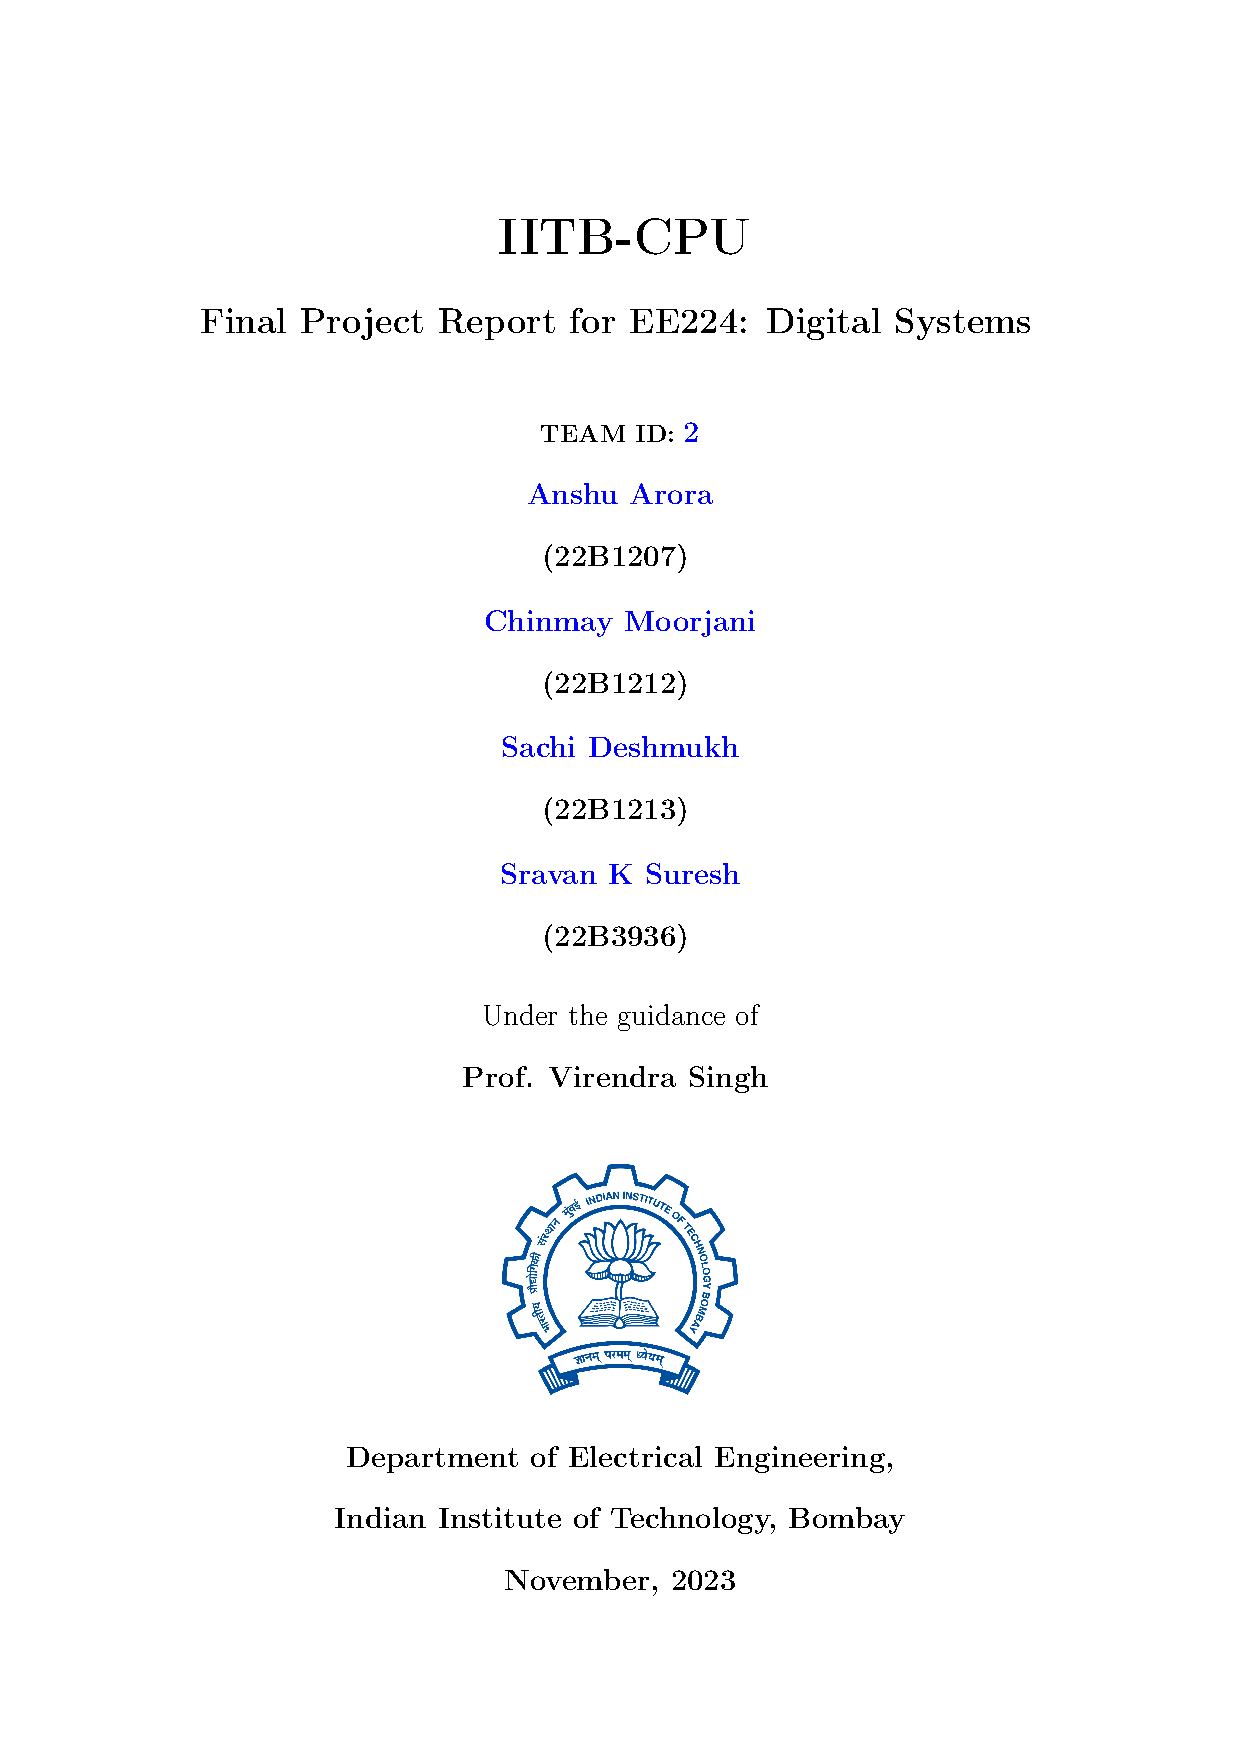
\includepdf[pages=-]{IITB_CPU_Report_CoverPage.pdf}

\maketitle
\tableofcontents
\newpage
\section{Introduction}
The IITB-CPU implements 14 instructions and utilises 8 programmer registers, among which the register 7 ($R7$) is used as a program counter or an instruction register. Internally, 17 states are used to implement these instructions and are described in the following section.

\section{Work Distribution}
\begin{table}[htb]
\centering
\begin{tabularx}{\textwidth}{|>{\centering\arraybackslash}X|>{\centering\arraybackslash}p{4cm}|}
\hline
\textbf{Tasks performed} & \textbf{Team member} \\ \hline
Ideation and Initial Design of Partial Datapaths for each Instruction                      & Chinmay Moorjani                     \\ \hline
Drawing Partial datapaths for each Instruction                                             & Sravan K Suresh                      \\ \hline
Listing the set of states for all instructions along with control signals for each state & Sachi Deshmukh                       \\ \hline
Elaboration of instruction flow for each of the individual states                          & Sachi Deshmukh                       \\ \hline
State reduction and pen-paper design of minimised FSM                                      & Chinmay Moorjani                     \\ \hline
Construction of final FSM using draw.io                                                    & Sravan K Suresh                      \\ \hline
Complete Datapath by merging the partial datapaths (Pen-paper design)                      & Chinmay Moorjani                     \\ \hline
Design and documentation of final Datapath using draw.io                                   & Anshu Arora                          \\ \hline
MUX tables that decide control flow                                                        & Anshu Arora                          \\ \hline
Output process/Control Signal table for every state                                        & Anshu Arora                          \\ \hline
Documentation of merging the entire CPU                                                    & Sachi Deshmukh                       \\ \hline
VHDL description of Multiplexers, Demultiplexers and Registers                             & Chinmay Moorjani and Sravan K Suresh \\ \hline
VHDL description of Register File                                                          & Sravan K Suresh and Anshu Arora      \\ \hline
VHDL description of ALU                                                                    & Sachi Deshmukh and Chinmay Moorjani  \\ \hline
VHDL description of Memory                                                                 & Chinmay Moorjani                     \\ \hline
VHDL realisation of CPU involving port mapping of components for Datapath            & Chinmay Moorjani                     \\ \hline
MUX processes and coding of FSM via clock, state-transition and o/p processes    & Chinmay Moorjani                     \\ \hline
Building Testbenches and TRACEFILES for each of the VHDL entities                                    & Sravan K Suresh                      \\ \hline
Cleaning, indentations and comments on all the VHDL codes                                      & Sravan K Suresh                      \\ \hline
Testing of Final CPU by hard-coded instructions in memory                                  & Chinmay Moorjani and Sravan K Suresh \\ \hline
Debugging and verification of Final CPU                                                    & Chinmay Moorjani and Sravan K Suresh       \\ \hline
Report drafting and document organisation                                                  & Sravan K Suresh                      \\ \hline
\end{tabularx}
\caption{Work Distribution Table}
\end{table}

Link to the GitHub repository of this project: \href{https://github.com/SRAVAN-IITB/EE224-Project}{\underline{Project Repository}}

\section{States}
\subsection*{Description}
The merged states and a short description of each is given below:
\begin{table}[!htb]
    \centering
\begin{tabular}{|
>{\columncolor[HTML]{96FFFB}}c |l|}
\hline
\cellcolor[HTML]{ECF4FF}\textbf{Merged States} & \cellcolor[HTML]{FFFFC7}\textbf{Function executed during the merged state} \\ \hline
\textbf{M1} & \begin{tabular}[c]{@{}l@{}}Fetch information and update instruction pointer (S1, S5, S9, S13, S17, \\ S21, S25, S29, S32, S35, S40, S44, S48, S52)\end{tabular} \\ \hline
\textbf{M2} & Understand and fetch operand (S2, S6, S10, S14, S18, S22, S26, S30, S33, S45, S49, S53) \\ \hline
\textbf{M3} & Execute operation (S3, S7, S11, S19, S23, S27) \\ \hline
\textbf{M4} & Update result (S4, S8, S12, S20, S24, S28) \\ \hline
\textbf{M5} & Execute addition operation (S15, S37, S42) \\ \hline
\textbf{M6} & Read memory (S38) \\ \hline
\textbf{M7} & Update register (S39) \\ \hline
\textbf{M8} & Store current instruction pointer (S50, S54) \\ \hline
\textbf{M9} & Store required value in specified location (S31) \\ \hline
\textbf{M10} & Store required value in specified location (S34) \\ \hline
\textbf{M11} & Read memory (S43) \\ \hline
\textbf{M12} & Compute Z (S46) \\ \hline
\textbf{M13} & If $z == 1$, then ip = ip+2+(imm6)×2 (S47) \\ \hline
\textbf{M14} & Compute and update IP (S51) \\ \hline
\textbf{M15} & Update IP (S55) \\ \hline
\textbf{M16} & Update result (S16) \\ \hline
\textbf{M17} & Understand and fetch operand (S36, S41) \\ \hline
\end{tabular}
    \caption{Description Table}
    \label{tab:desc}
\end{table}



\subsection{State Diagram}
      \begin{center}
          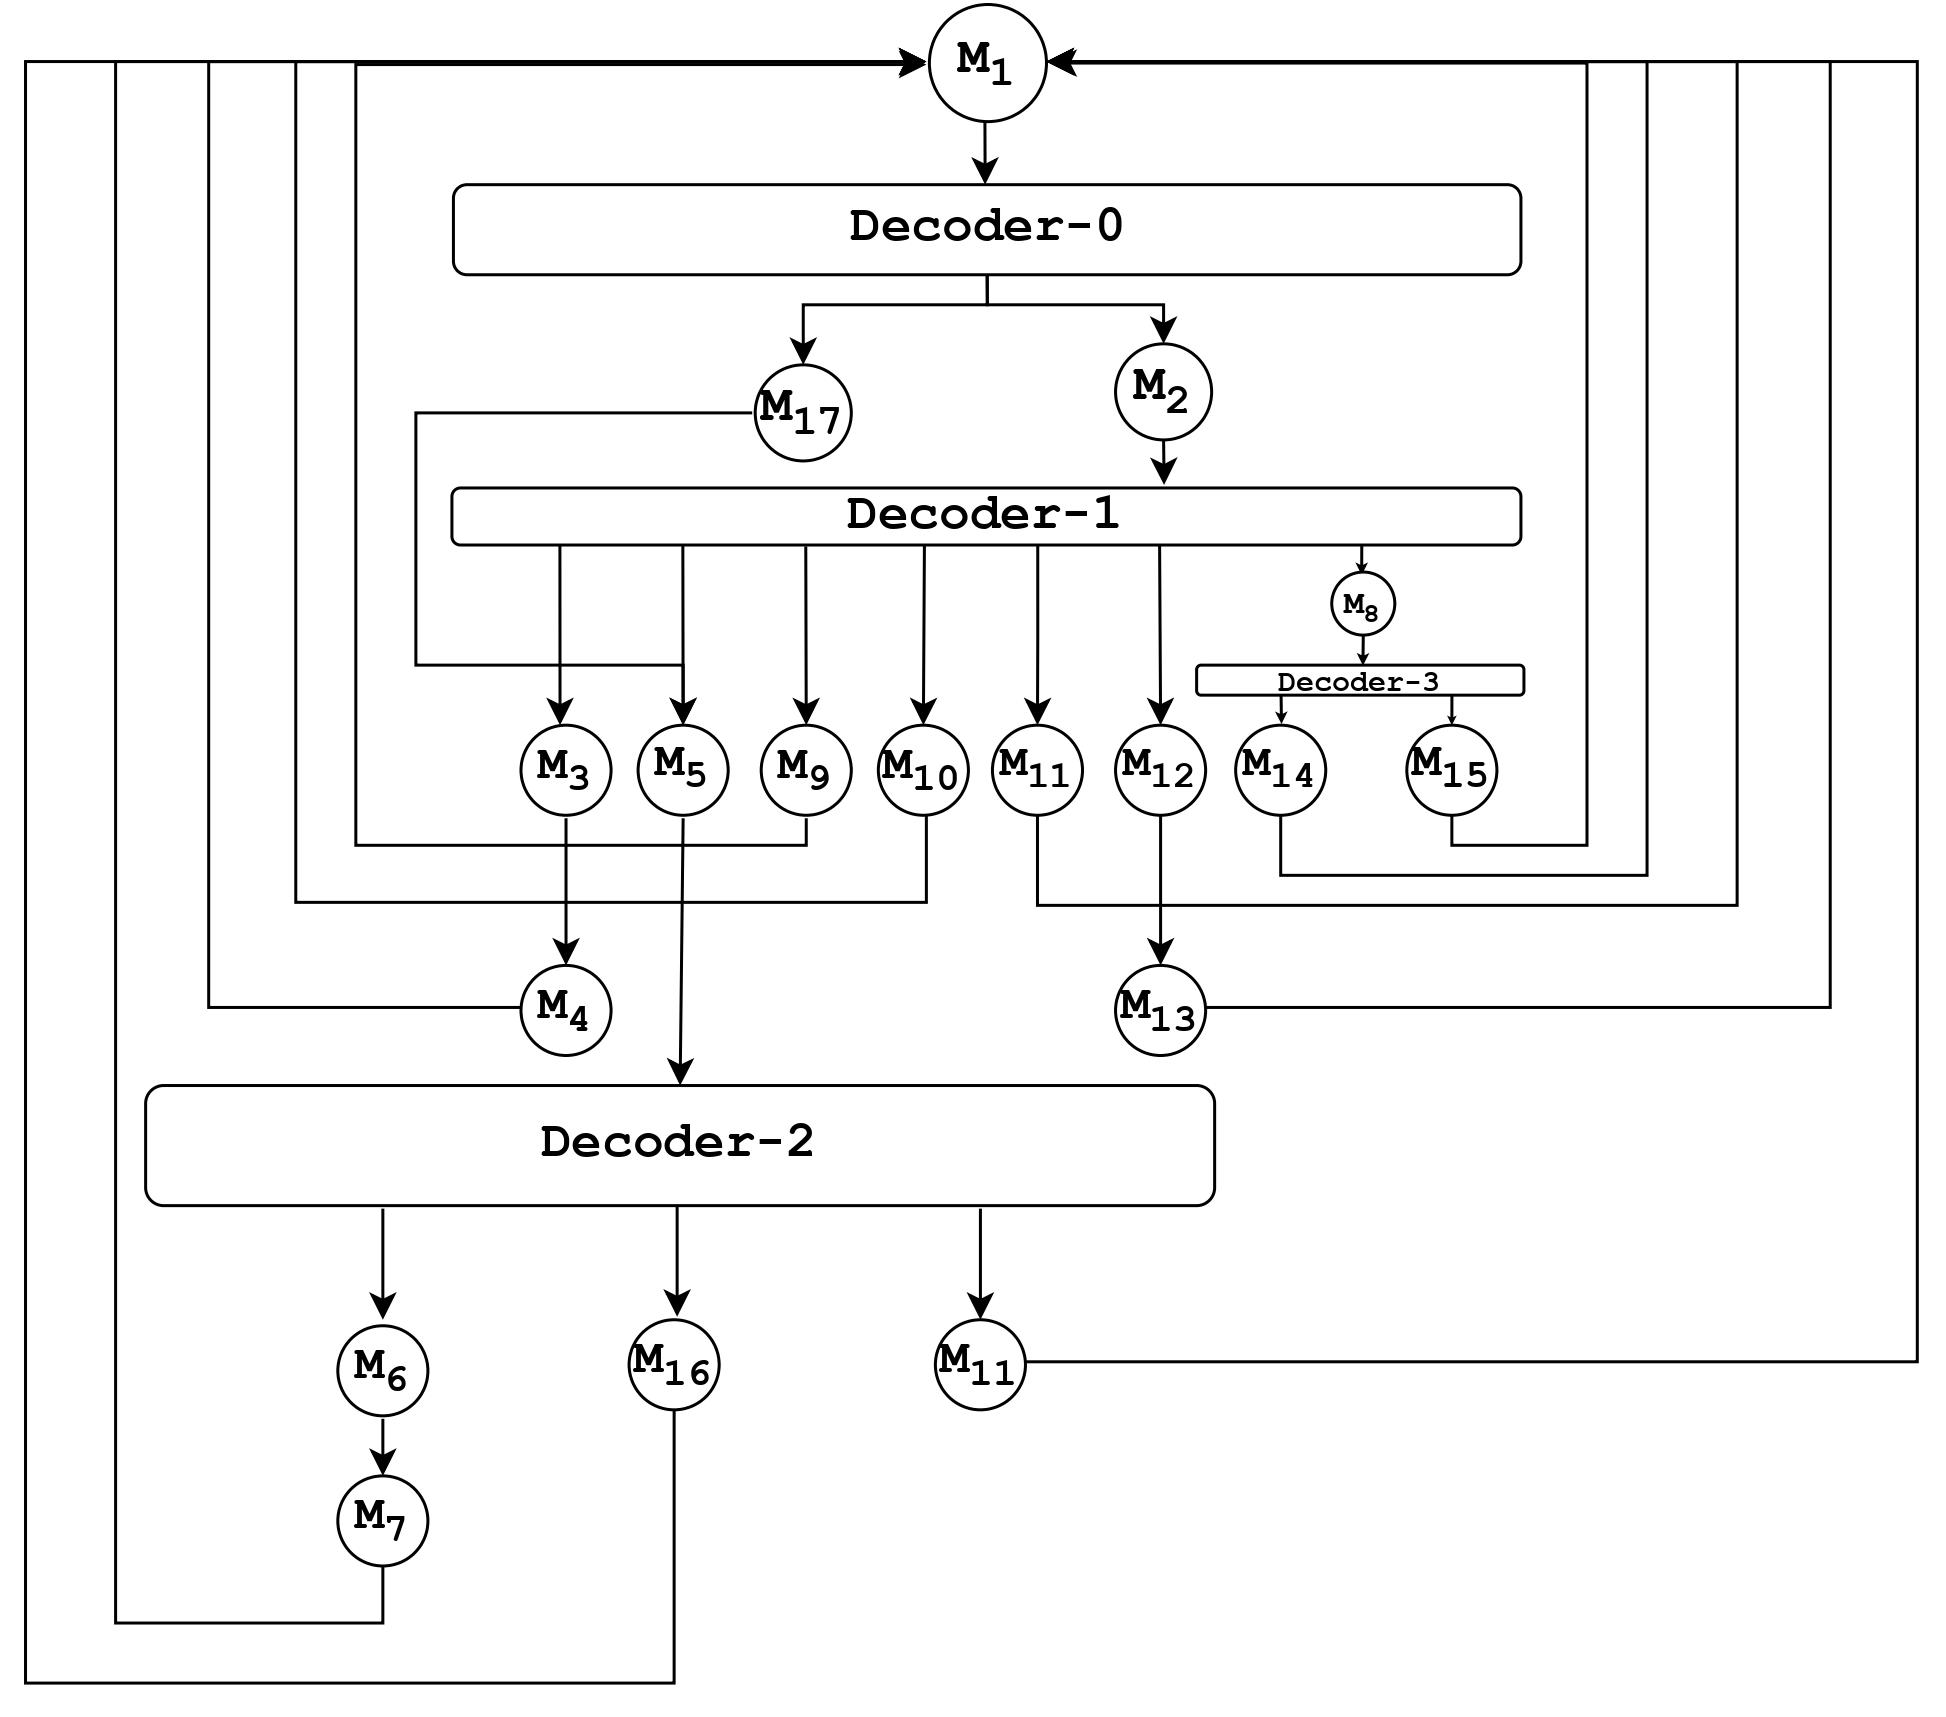
\includegraphics[width = 1.02\linewidth]{Images/fsm.jpg}
      \end{center}

\subsection{Components of IITB-CPU Design}
    \begin{center}
          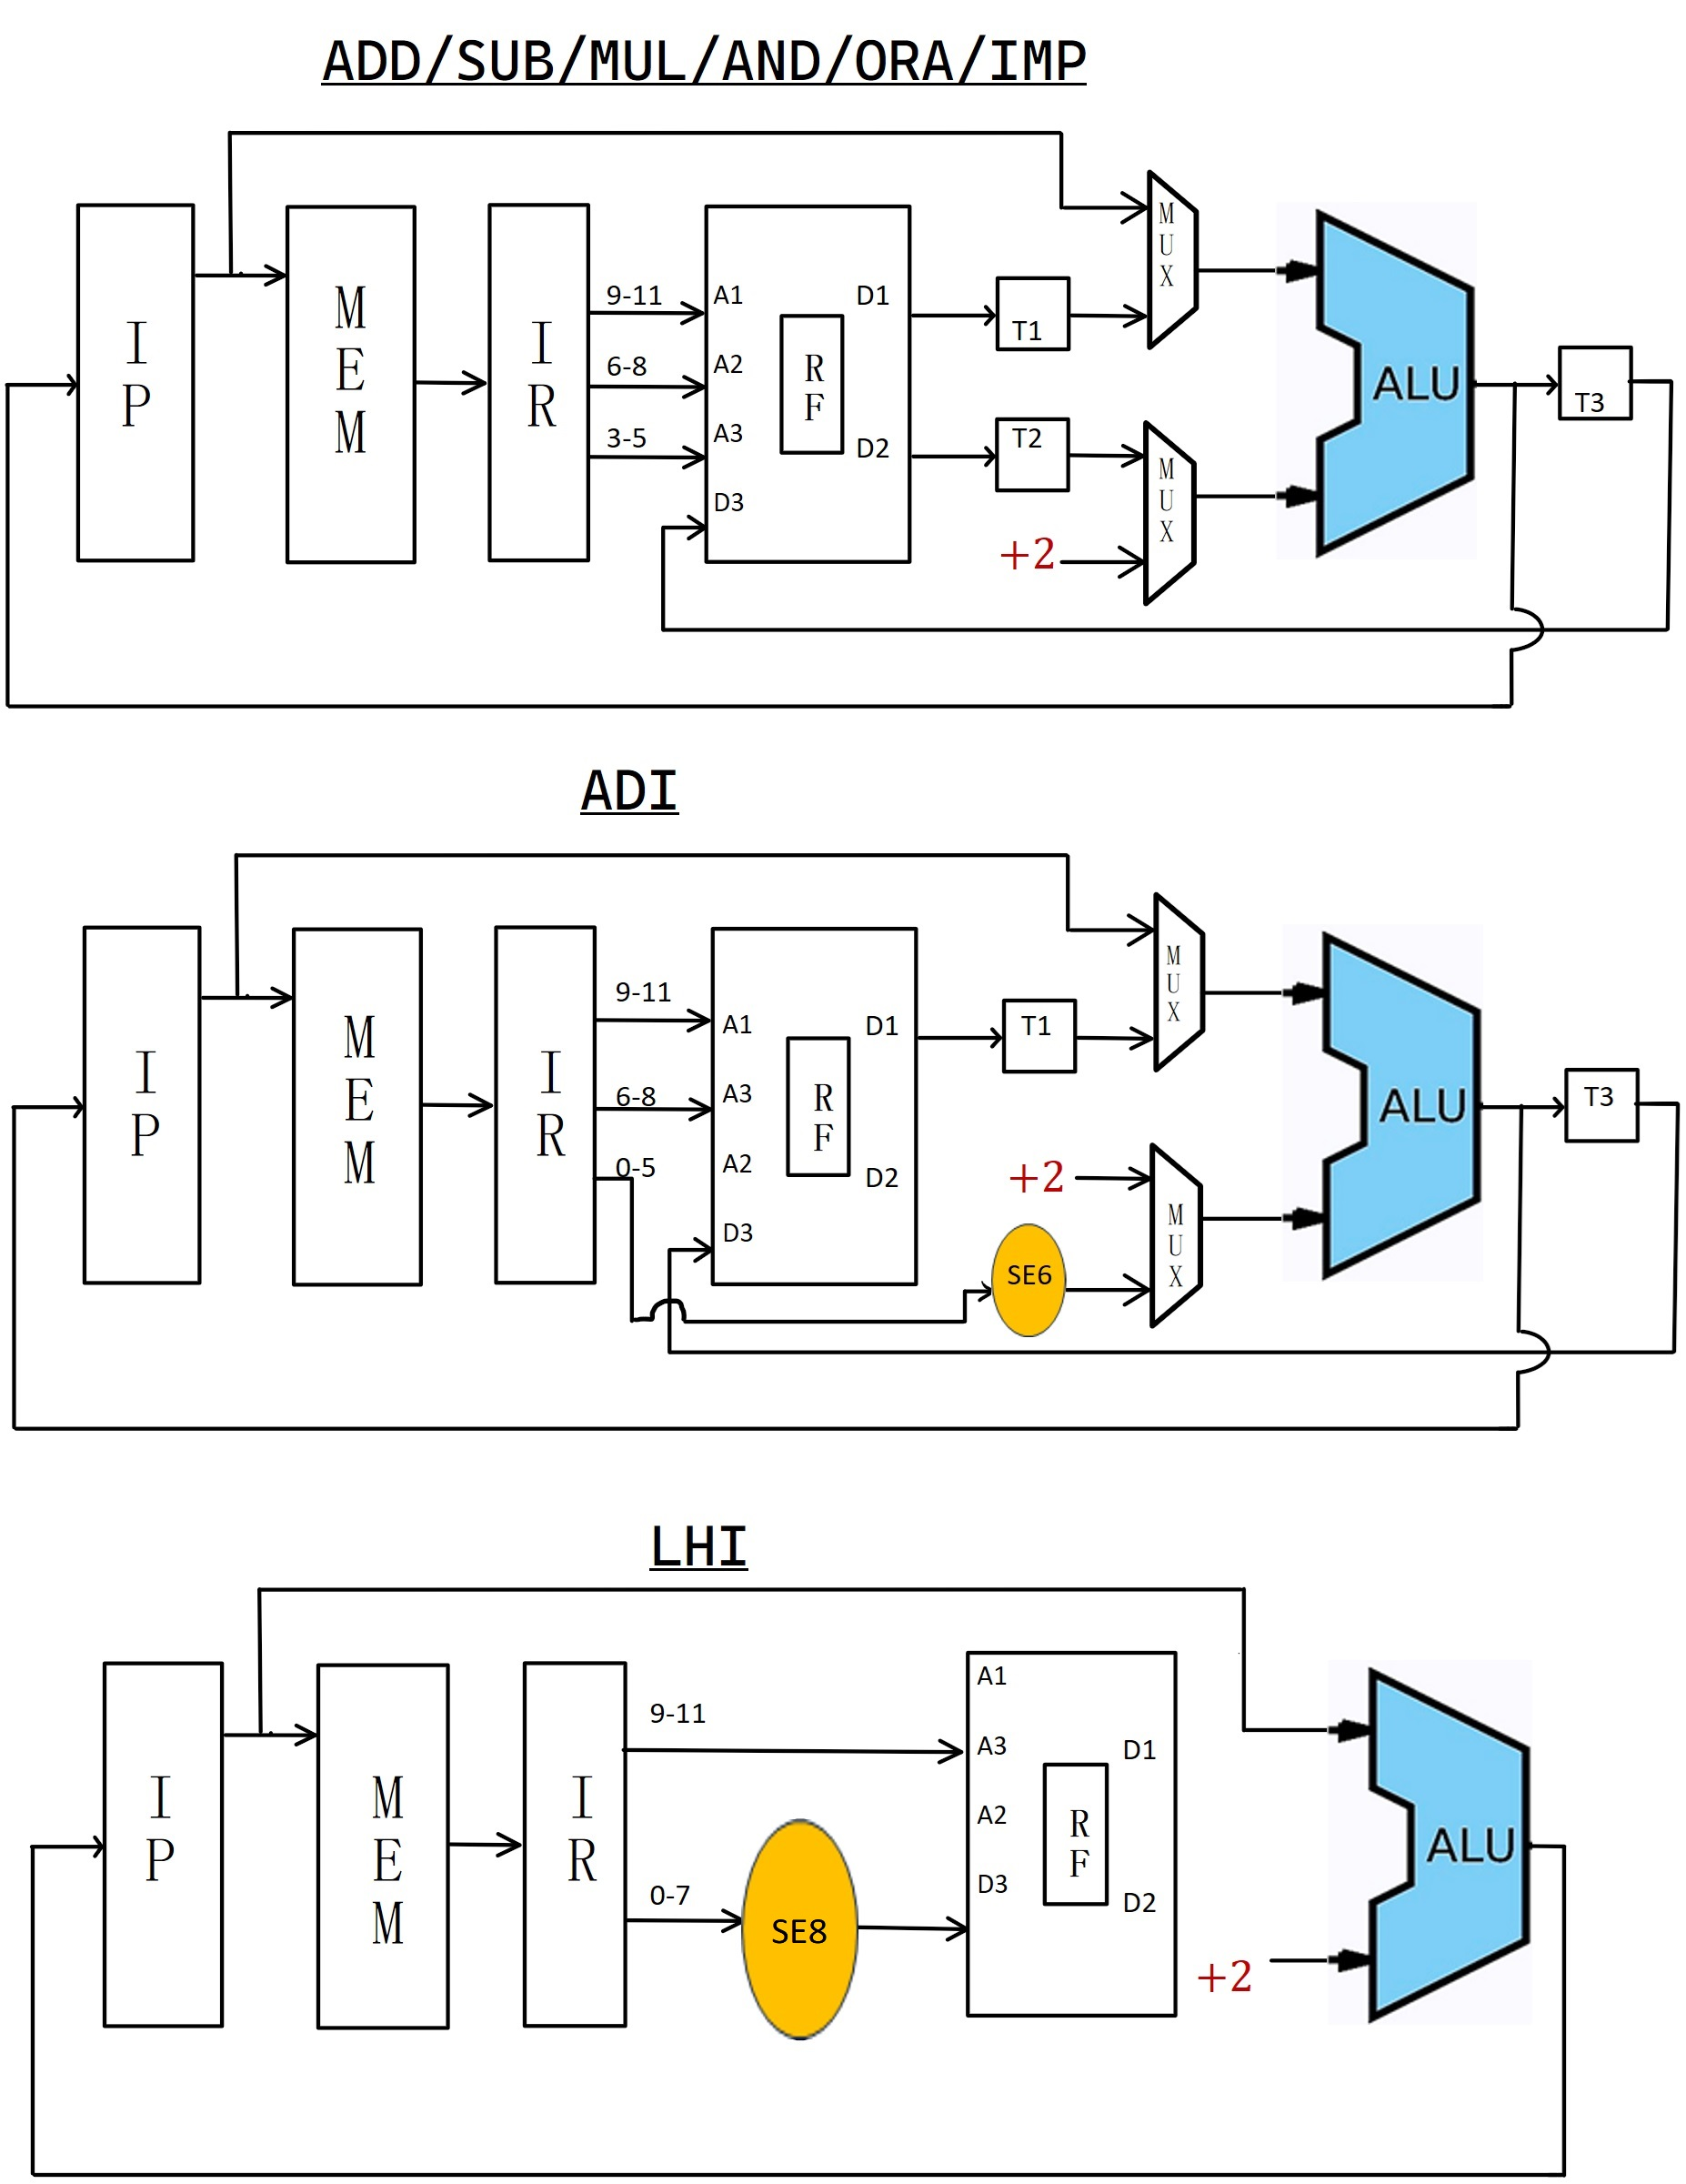
\includegraphics[width = 0.99\linewidth]{Images/1.jpg}
      \end{center}
    \begin{center}
          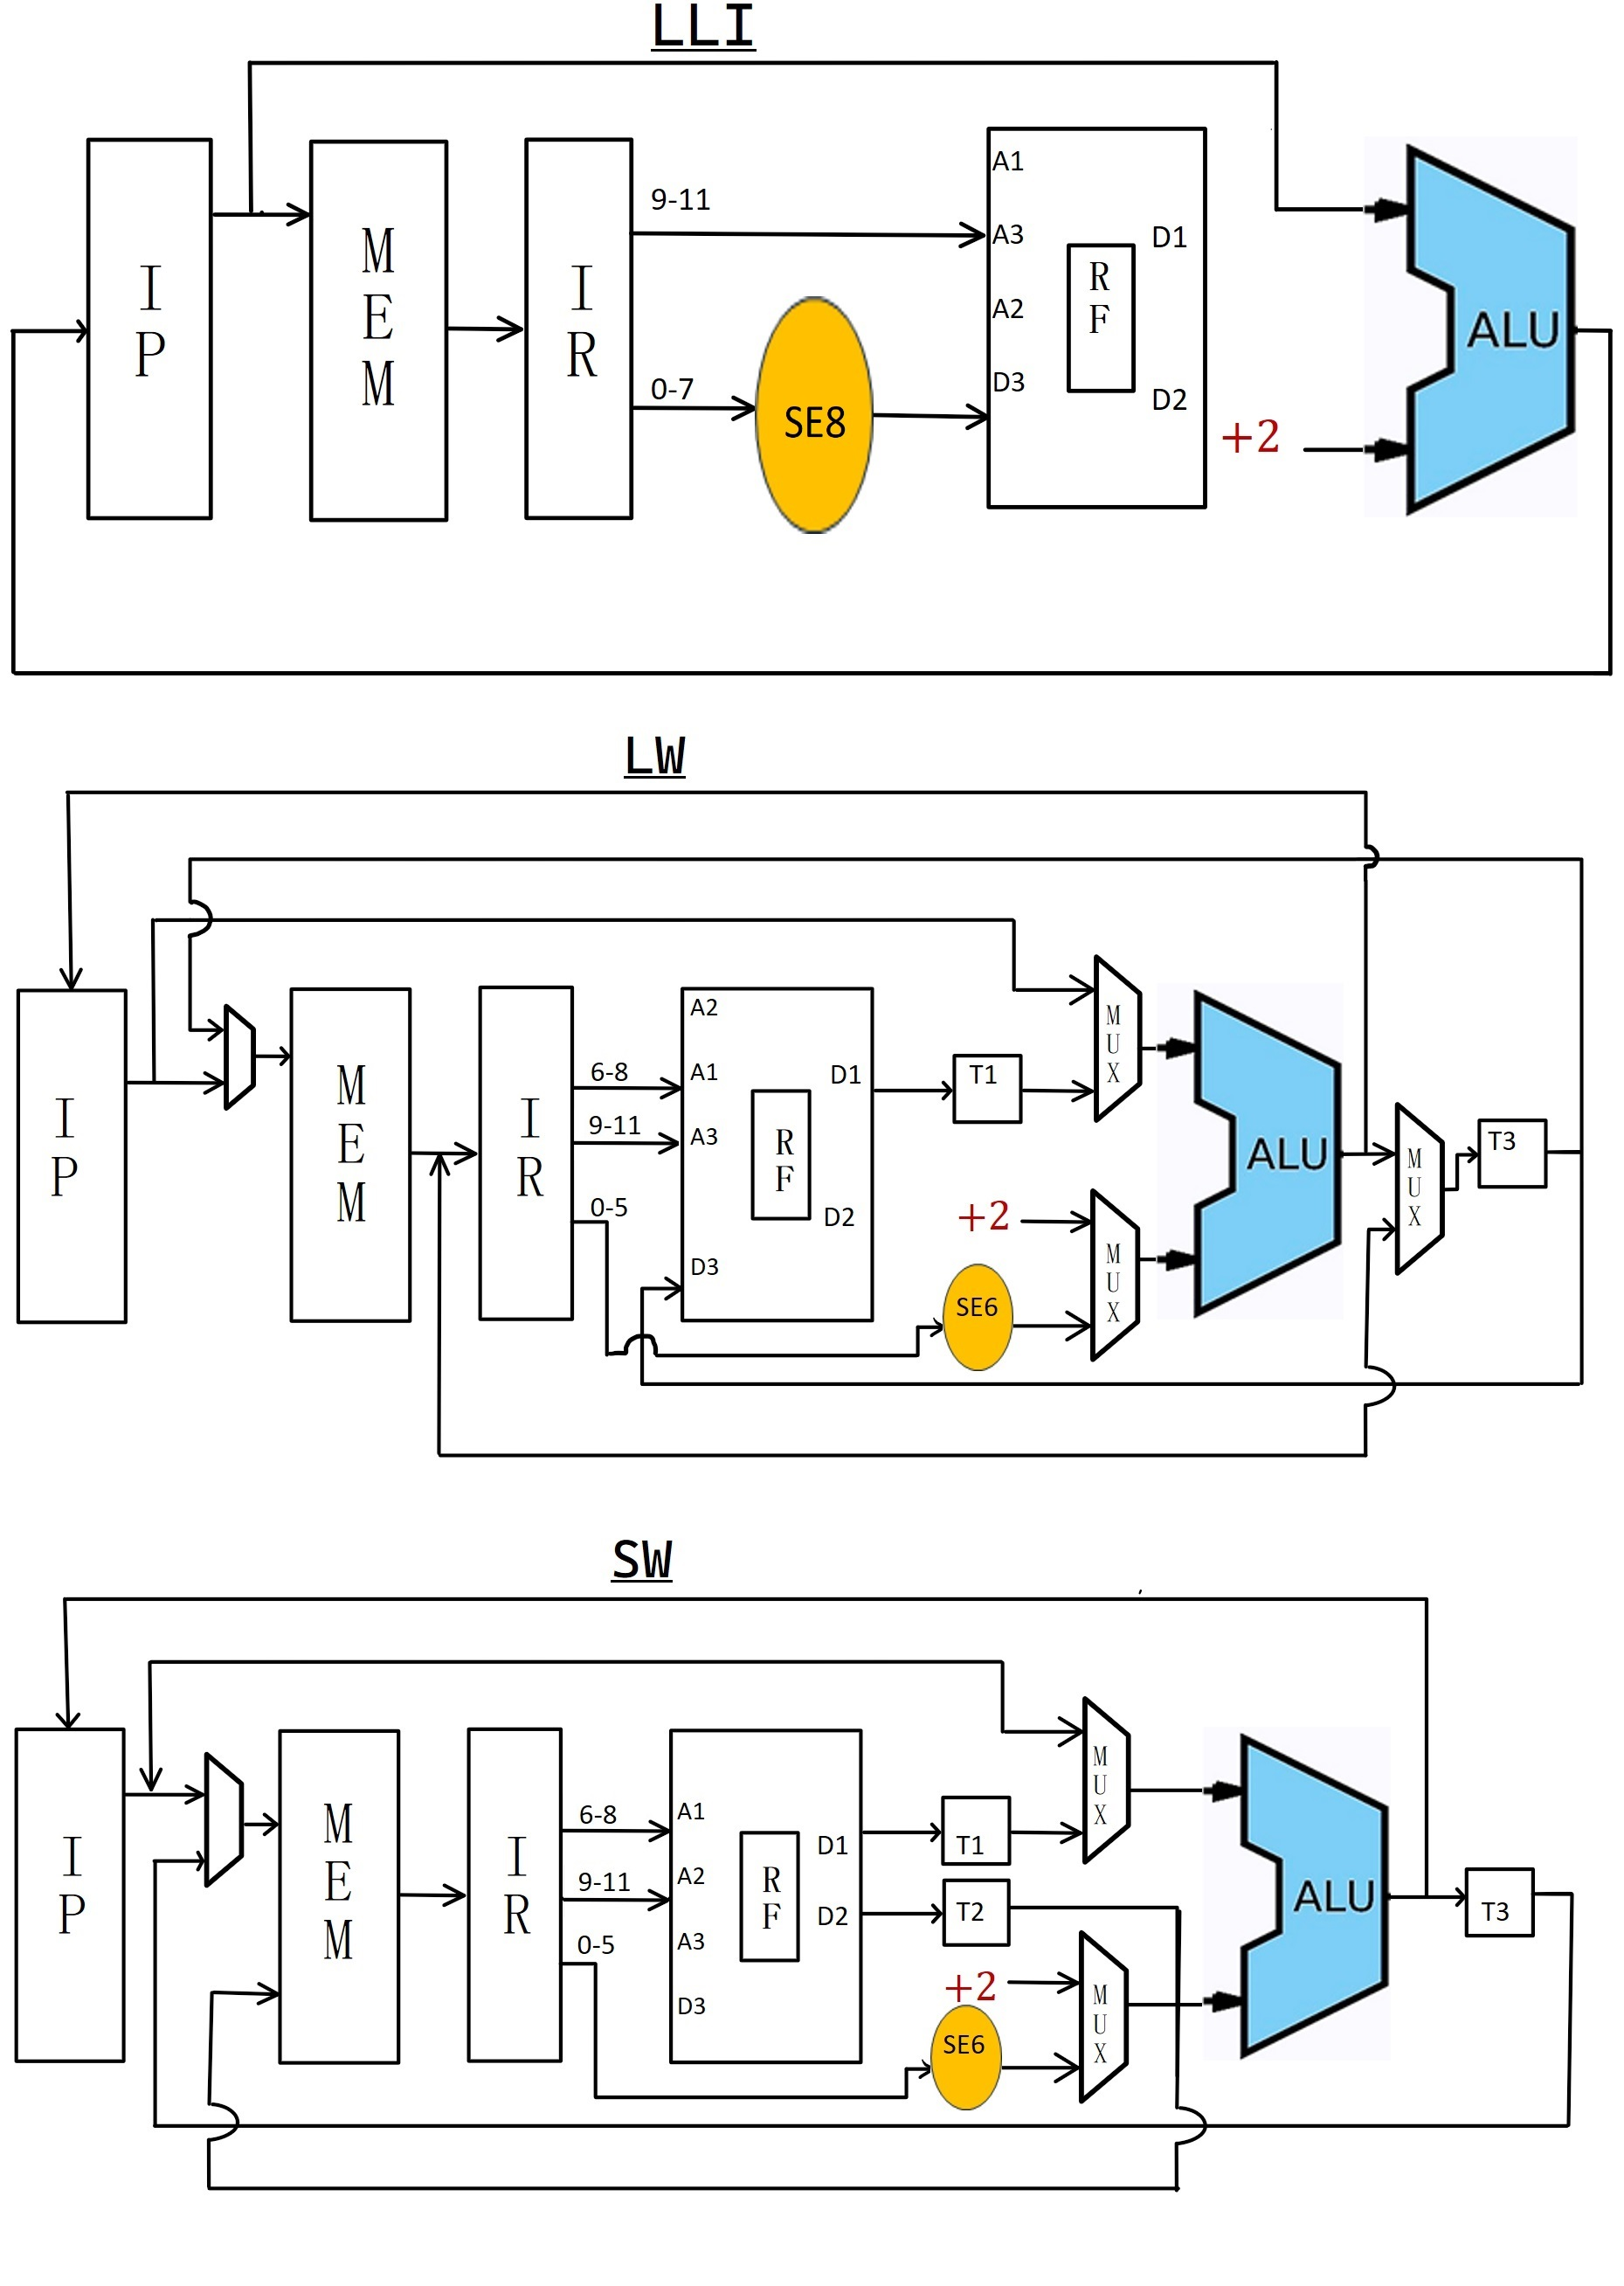
\includegraphics[width = 0.99\linewidth]{Images/2.jpg}
      \end{center}
    \begin{center}
          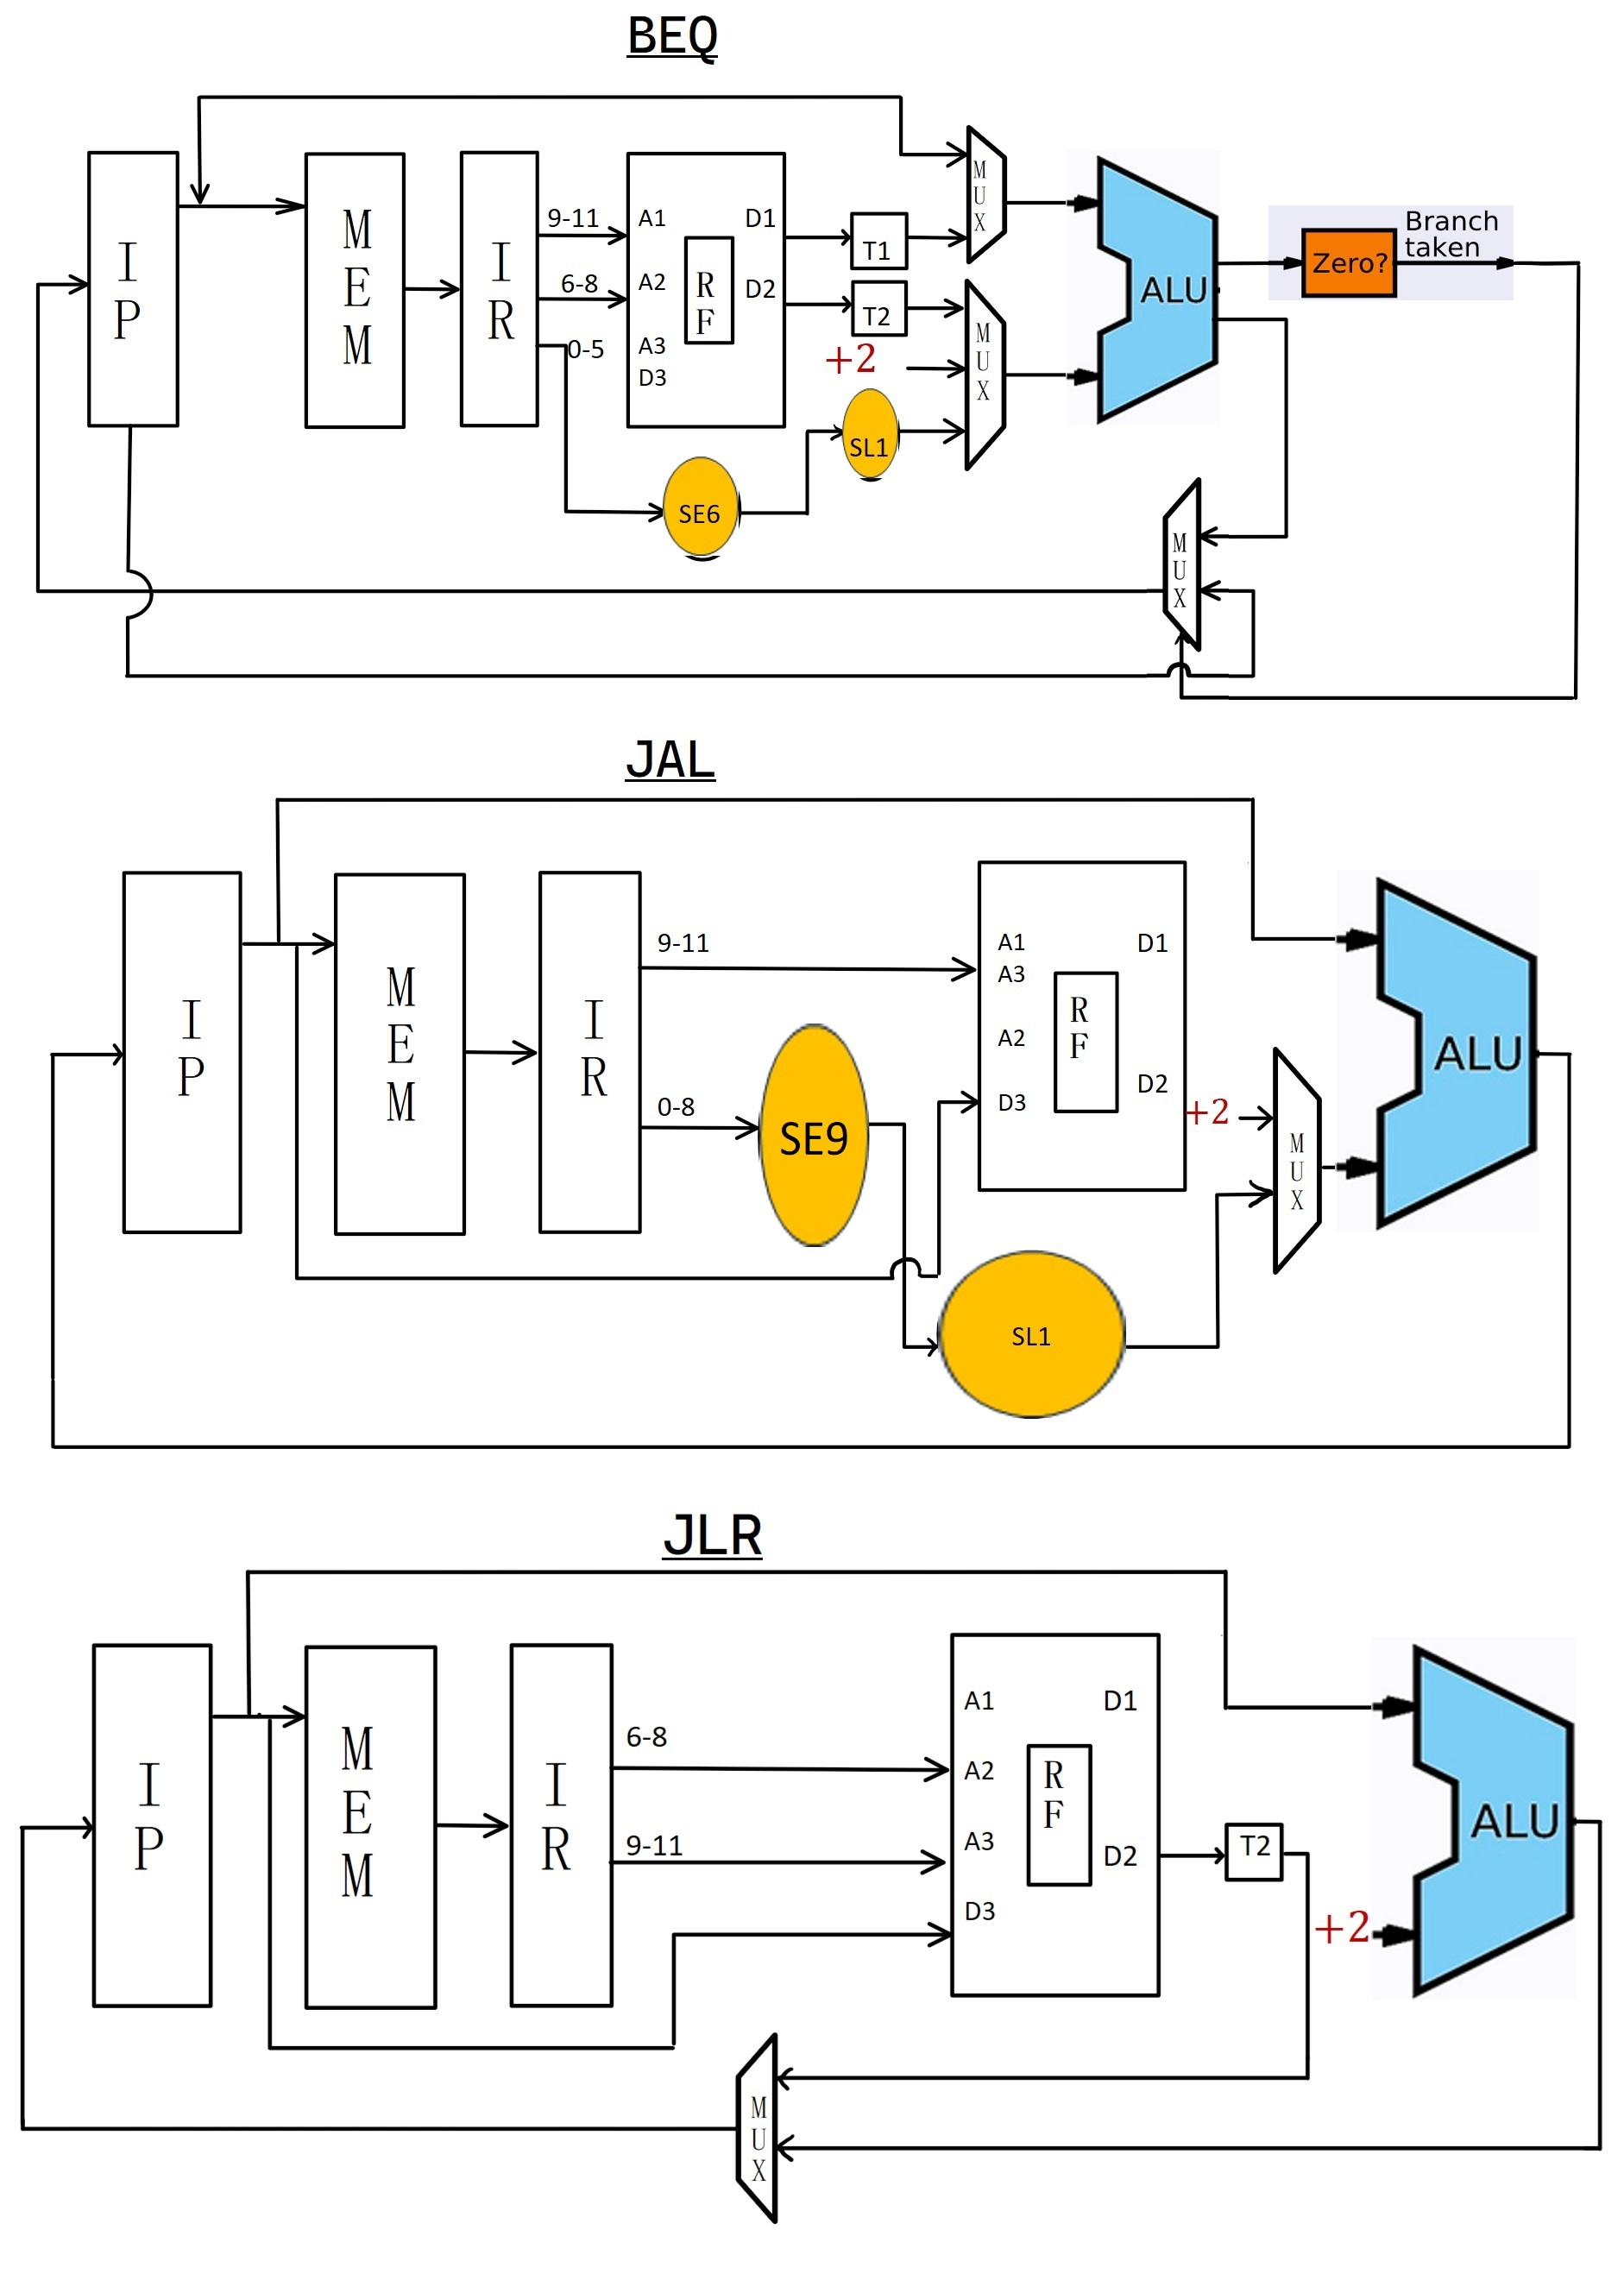
\includegraphics[width = 0.99\linewidth]{Images/3.jpg}
      \end{center}
\section{MUX Tables and Final Datapath of CPU}

\begin{table}[htb]
\centering
\begin{tabular}{|c|c|c|}
\hline
\rowcolor[HTML]{FFFC9E} 
\textbf{B1}                       & \textbf{B0}                       & \textbf{OUTPUT   SELECTED}         \\ \hline
{\color[HTML]{680100} \textbf{0}} & {\color[HTML]{680100} \textbf{0}} & {\color[HTML]{013300} Do Nothing}  \\ \hline
{\color[HTML]{680100} \textbf{0}} & {\color[HTML]{680100} \textbf{1}} & {\color[HTML]{013300} Addition}    \\ \hline
{\color[HTML]{680100} \textbf{1}} & {\color[HTML]{680100} \textbf{0}} & {\color[HTML]{013300} Subtraction} \\ \hline
{\color[HTML]{680100} \textbf{1}} & {\color[HTML]{680100} \textbf{1}} & {\color[HTML]{013300} IR 12\_15}   \\ \hline
\end{tabular}
\caption{Table of \textbf{MUX-1}}
\end{table}

\begin{table}[htb]
\centering
\begin{tabular}{|c|c|c|}
\hline
\rowcolor[HTML]{FFFC9E} 
\textbf{B3}                       & \textbf{B2}                       & \textbf{OUTPUT   SELECTED}        \\ \hline
{\color[HTML]{680100} \textbf{0}} & {\color[HTML]{680100} \textbf{0}} & {\color[HTML]{013300} Do Nothing} \\ \hline
{\color[HTML]{680100} \textbf{0}} & {\color[HTML]{680100} \textbf{1}} & {\color[HTML]{013300} IR 3\_5}    \\ \hline
{\color[HTML]{680100} \textbf{1}} & {\color[HTML]{680100} \textbf{0}} & {\color[HTML]{013300} IR 6\_8}    \\ \hline
{\color[HTML]{680100} \textbf{1}} & {\color[HTML]{680100} \textbf{1}} & {\color[HTML]{013300} IR 9\_11}   \\ \hline
\end{tabular}
\caption{Table of \textbf{MUX-2}}
\end{table}

\begin{table}[htb]
\centering
\begin{tabular}{|c|c|c|c|}
\hline
\rowcolor[HTML]{FFFC9E} 
\textbf{B6}                       & \textbf{B5}                       & \textbf{B4}                       & OUTPUT   SELECTED                           \\ \hline
{\color[HTML]{680100} \textbf{0}} & {\color[HTML]{680100} \textbf{0}} & {\color[HTML]{680100} \textbf{0}} & {\color[HTML]{013300} Do Nothing}           \\ \hline
{\color[HTML]{680100} \textbf{0}} & {\color[HTML]{680100} \textbf{0}} & {\color[HTML]{680100} \textbf{1}} & {\color[HTML]{013300} T3}                   \\ \hline
{\color[HTML]{680100} \textbf{0}} & {\color[HTML]{680100} \textbf{1}} & {\color[HTML]{680100} \textbf{0}} & {\color[HTML]{013300} IR 0\_7 $\rightarrow$   SE8 Right} \\ \hline
{\color[HTML]{680100} \textbf{0}} & {\color[HTML]{680100} \textbf{1}} & {\color[HTML]{680100} \textbf{1}} & {\color[HTML]{013300} IR 0\_7 $\rightarrow$   SE8 Left}  \\ \hline
{\color[HTML]{680100} \textbf{1}} & {\color[HTML]{680100} \textbf{0}} & {\color[HTML]{680100} \textbf{0}} & {\color[HTML]{013300} IP}                   \\ \hline
{\color[HTML]{680100} \textbf{1}} & {\color[HTML]{680100} \textbf{0}} & {\color[HTML]{680100} \textbf{1}} & {\color[HTML]{013300} M8}                   \\ \hline
\end{tabular}
\caption{Table of \textbf{MUX-3}}
\end{table}

\begin{table}[htb]
\centering
\begin{tabular}{|c|c|c|}
\hline
\rowcolor[HTML]{FFFC9E} 
\textbf{B8}                       & \textbf{B7}                       & \textbf{OUTPUT   SELECTED}        \\ \hline
{\color[HTML]{680100} \textbf{0}} & {\color[HTML]{680100} \textbf{0}} & {\color[HTML]{013300} Do Nothing} \\ \hline
{\color[HTML]{680100} \textbf{0}} & {\color[HTML]{680100} \textbf{1}} & {\color[HTML]{013300} IP}         \\ \hline
{\color[HTML]{680100} \textbf{1}} & {\color[HTML]{680100} \textbf{0}} & {\color[HTML]{013300} T1}         \\ \hline
{\color[HTML]{680100} \textbf{0}} & {\color[HTML]{680100} \textbf{1}} & {\color[HTML]{013300} 1}          \\ \hline
\end{tabular}
\caption{Table of \textbf{MUX-4}}
\end{table}

\begin{table}[htb]
\centering
\begin{tabular}{|c|c|c|c|}
\hline
\rowcolor[HTML]{FFFC9E} 
\textbf{B11}                      & \textbf{B10}                      & \textbf{B9}                       & \textbf{OUTPUT   SELECTED}         \\ \hline
{\color[HTML]{680100} \textbf{0}} & {\color[HTML]{680100} \textbf{0}} & {\color[HTML]{680100} \textbf{0}} & {\color[HTML]{013300} Do Nothing}  \\ \hline
{\color[HTML]{680100} \textbf{0}} & {\color[HTML]{680100} \textbf{0}} & {\color[HTML]{680100} \textbf{1}} & {\color[HTML]{013300} +2}          \\ \hline
{\color[HTML]{680100} \textbf{0}} & {\color[HTML]{680100} \textbf{1}} & {\color[HTML]{680100} \textbf{0}} & {\color[HTML]{013300} T2}          \\ \hline
{\color[HTML]{680100} \textbf{0}} & {\color[HTML]{680100} \textbf{1}} & {\color[HTML]{680100} \textbf{1}} & {\color[HTML]{013300} SE6}         \\ \hline
{\color[HTML]{680100} \textbf{1}} & {\color[HTML]{680100} \textbf{0}} & {\color[HTML]{680100} \textbf{0}} & {\color[HTML]{013300} SE6 $\rightarrow$   LS1} \\ \hline
{\color[HTML]{680100} \textbf{1}} & {\color[HTML]{680100} \textbf{0}} & {\color[HTML]{680100} \textbf{1}} & {\color[HTML]{013300} SE9}         \\ \hline
\end{tabular}
\caption{Table of \textbf{MUX-5}}
\end{table}

\begin{table}[htb]
\centering
\begin{tabular}{|c|c|c|c|}
\hline
\rowcolor[HTML]{FFFC9E} 
\textbf{B13}                      & \textbf{B12}                      & \textbf{OUTPUT   SELECTED}        \\ \hline
{\color[HTML]{680100} \textbf{0}} & {\color[HTML]{680100} \textbf{0}} & {\color[HTML]{013300} Do Nothing} \\ \hline
{\color[HTML]{680100} \textbf{0}} & {\color[HTML]{680100} \textbf{1}} & {\color[HTML]{013300} IP}         \\ \hline
{\color[HTML]{680100} \textbf{1}} & {\color[HTML]{680100} \textbf{0}} & {\color[HTML]{013300} T3}         \\ \hline
\end{tabular}
\caption{Table of \textbf{MUX-6}}
\end{table}

\begin{table}[htb]
\centering
\begin{tabular}{|c|c|c|}
\hline
\rowcolor[HTML]{FFFC9E} 
\textbf{B15}                      & \textbf{B14}                      & \textbf{OUTPUT   SELECTED}           \\ \hline
{\color[HTML]{680100} \textbf{0}} & {\color[HTML]{680100} \textbf{0}} & {\color[HTML]{013300} Do Nothing}    \\ \hline
{\color[HTML]{680100} \textbf{0}} & {\color[HTML]{680100} \textbf{1}} & {\color[HTML]{013300} ALU\_C}        \\ \hline
{\color[HTML]{680100} \textbf{1}} & {\color[HTML]{680100} \textbf{0}} & {\color[HTML]{013300} Memory   Data} \\ \hline
\end{tabular}
\caption{Table of \textbf{MUX-7}}
\end{table}

\begin{table}[htb]
\centering
\begin{tabular}{|c|c|c|}
\hline
\rowcolor[HTML]{FFFC9E} 
\textbf{B17}                      & \textbf{B16}                      & \textbf{OUTPUT   SELECTED}        \\ \hline
{\color[HTML]{680100} \textbf{0}} & {\color[HTML]{680100} \textbf{0}} & {\color[HTML]{013300} Do Nothing} \\ \hline
{\color[HTML]{680100} \textbf{0}} & {\color[HTML]{680100} \textbf{1}} & {\color[HTML]{013300} ALU\_C}     \\ \hline
{\color[HTML]{680100} \textbf{1}} & {\color[HTML]{680100} \textbf{0}} & {\color[HTML]{013300} BEQ}        \\ \hline
{\color[HTML]{680100} \textbf{1}} & {\color[HTML]{680100} \textbf{1}} & {\color[HTML]{013300} T2}         \\ \hline
\end{tabular}
\caption{Table of \textbf{MUX-8}}
\end{table}

\begin{table}[htb]
\centering
\begin{tabular}{|c|c|c|}
\hline
\rowcolor[HTML]{FFFC9E} 
\textbf{B18}                      & \textbf{OUTPUT   SELECTED}      \\ \hline
{\color[HTML]{680100} \textbf{0}} & {\color[HTML]{013300} IR 9\_11} \\ \hline
{\color[HTML]{680100} \textbf{1}} & {\color[HTML]{013300} IR 6\_8}  \\ \hline
\end{tabular}
\caption{Table of \textbf{MUX-9}}
\end{table}

\begin{table}[htb]
\centering
\begin{tabular}{|c|c|c|}
\hline
\rowcolor[HTML]{FFFC9E} 
\textbf{B19}                      & \textbf{OUTPUT   SELECTED}      \\ \hline
{\color[HTML]{680100} \textbf{0}} & {\color[HTML]{013300} IR 6\_8}  \\ \hline
{\color[HTML]{680100} \textbf{1}} & {\color[HTML]{013300} IR 9\_11} \\ \hline
\end{tabular}
\caption{Table of \textbf{MUX-10}}
\end{table}

\clearpage
\section{Control Signal table}
\begin{table}[!htb]
\setlength{\tabcolsep}{4pt} % Adjust horizontal spacing between columns
\begin{tabular}
{{|>{\columncolor{cyan}}c|c|c|c|c|c|c|c|c|c|c|c|c|c|c|c|c|c|c|c|c|c|}}
\hline
\rowcolor{yellow} % Color the first row orange
\textbf{X to} & \textbf{B19} & \textbf{B18} & \textbf{B17} & \textbf{B16} & \textbf{B15} & \textbf{B14} & \textbf{B13} & \textbf{B12} & \textbf{B11} & \textbf{B10} & \textbf{B9} & \textbf{B8} & \textbf{B7} & \textbf{B6} & \textbf{B5} & \textbf{B4} & \textbf{B3} & \textbf{B2} & \textbf{B1} & \textbf{B0} \\ \hline
\textbf{M1} & 0 & 0 & 0 & 1 & 0 & 0 & 0 & 1 & 0 & 0 & 1 & 0 & 1 & 1 & 0 & 1 & 0 & 0 & 0 & 1 \\ \hline
\textbf{M2} & 0 & 0 & 0 & 0 & 0 & 0 & 0 & 0 & 0 & 0 & 0 & 0 & 0 & 0 & 0 & 0 & 0 & 0 & 0 & 0 \\ \hline
\textbf{M3} & 0 & 0 & 0 & 0 & 0 & 1 & 0 & 0 & 0 & 1 & 0 & 1 & 0 & 0 & 0 & 0 & 0 & 0 & 1 & 1 \\ \hline
\textbf{M4} & 0 & 0 & 0 & 0 & 0 & 0 & 0 & 0 & 0 & 0 & 0 & 0 & 0 & 0 & 0 & 1 & 0 & 1 & 0 & 0 \\ \hline
\textbf{M5} & 0 & 0 & 0 & 0 & 0 & 1 & 0 & 0 & 0 & 1 & 1 & 1 & 0 & 0 & 0 & 0 & 0 & 0 & 0 & 0 \\ \hline
\textbf{M6} & 0 & 0 & 0 & 0 & 1 & 0 & 1 & 0 & 0 & 0 & 0 & 0 & 0 & 0 & 0 & 0 & 0 & 0 & 0 & 0 \\ \hline
\textbf{M7} & 0 & 0 & 0 & 0 & 0 & 0 & 0 & 0 & 0 & 0 & 0 & 0 & 0 & 0 & 0 & 1 & 1 & 1 & 0 & 0 \\ \hline
\textbf{M8} & 0 & 0 & 0 & 0 & 0 & 0 & 0 & 0 & 0 & 0 & 0 & 0 & 0 & 1 & 0 & 0 & 1 & 1 & 0 & 0 \\ \hline
\textbf{M9} & 0 & 0 & 0 & 0 & 0 & 0 & 0 & 0 & 0 & 0 & 0 & 0 & 0 & 0 & 1 & 0 & 1 & 1 & 0 & 0 \\ \hline
\textbf{M10} & 0 & 0 & 0 & 0 & 0 & 0 & 0 & 0 & 0 & 0 & 0 & 0 & 0 & 0 & 1 & 1 & 1 & 1 & 0 & 0 \\ \hline
\textbf{M11} & 0 & 0 & 0 & 0 & 0 & 0 & 1 & 0 & 0 & 0 & 0 & 0 & 0 & 0 & 0 & 0 & 0 & 0 & 0 & 0 \\ \hline
\textbf{M12} & 0 & 0 & 0 & 0 & 0 & 0 & 0 & 0 & 0 & 1 & 0 & 1 & 0 & 0 & 0 & 0 & 0 & 0 & 1 & 0 \\ \hline
\textbf{M13} & 0 & 0 & 1 & 0 & 0 & 0 & 0 & 0 & 1 & 0 & 0 & 0 & 1 & 1 & 0 & 1 & 0 & 0 & 0 & 1 \\ \hline
\textbf{M14} & 0 & 0 & 0 & 1 & 0 & 0 & 0 & 0 & 1 & 0 & 1 & 0 & 1 & 1 & 0 & 1 & 0 & 0 & 0 & 1 \\ \hline
\textbf{M15} & 0 & 0 & 1 & 1 & 0 & 0 & 0 & 0 & 0 & 0 & 0 & 0 & 0 & 1 & 0 & 1 & 0 & 0 & 0 & 0 \\ \hline
\textbf{M16} & 0 & 0 & 0 & 0 & 0 & 0 & 0 & 0 & 0 & 0 & 0 & 0 & 0 & 0 & 0 & 1 & 1 & 0 & 0 & 0 \\ \hline
\textbf{M17} & 1 & 1 & 0 & 0 & 0 & 0 & 0 & 0 & 0 & 0 & 0 & 0 & 0 & 0 & 0 & 0 & 0 & 0 & 0 & 0 \\ \hline
\end{tabular}
\caption{Output process/Control Signal table for every state}
\end{table}

\\~\\
In the implementation of a Finite State Machine (FSM), multiple Multiplexers (MUX) are employed to regulate signal flow and manage the execution of operations. The system comprises 17 MUX units, collectively featuring 20 select lines. Altering the control signal proves instrumental in facilitating state transitions.\\


\clearpage
\newpage

\section{Testing}
\subsection{Condensed code of CPU.vhdl}
The code below is a condensed version of our VHDL description of CPU with only \texttt{clk} and \texttt{reset} as input signals.
\begin{lstlisting}
library IEEE;
use IEEE.std_logic_1164.all;

entity CPU is
    port (
        Clk, Reset: in std_logic
    );
end entity CPU;

architecture struct of CPU is

    type state is (rst, S1, S2, S3, S4, S5, S6, S7, S8, S9, S10, S11, S12, S13, S14, S15, S16, S17);
    -- Declaration of components Reg_File, MUX_8, MUX_4, MUX_2, Memory, ALU
    component Reg_File is 
    {...}
    end component;
    component MUX_8 is 
    {...}
    end component;
    component MUX_4 is 
    {...}
    end component;
    component MUX_2 is 
    {...}
    end component;
    component Memory is 
    {...}
    end component;
    component ALU is 
    {...}
    end component;

    signal M2, M9, M10: std_logic_vector(2 downto 0);
    signal M1: std_logic_vector(3 downto 0);
    signal Mem_W, Mem_R, Z_flag, T1_W, T2_W, IP_store: std_logic;
    signal B: std_logic_vector(19 downto 0);
    signal state_present, state_next: state := rst;
    
begin

    Program_Counter: Reg_16BIT port map (Clk => Clk, 
															Reset => Reset, 
															data_in => M8, 
															data_out => IP);
															
    MyMemory: Memory port map (Address => M6, 
										data_write => T2_data, 
										data_out => Mem_data, 
										clock => clk, 
										MeM_W => Mem_W, 
										MeM_R => Mem_R);
										
    Instruction_Register: Reg_16BIT port map (Reset => Reset, 
																Clk => clk, 
																data_in => Mem_data, 
																data_out => IR);
																
    Reg_File1 : Reg_File port map (Clk   => Clk,
											  Reset => Reset, 
									Address_Read1 => M9, 
									Address_Read2 => M10, 
									Address_Write => M2, 
										data_Write => M3, 
										data_Read1 => DataA, 
										data_Read2 => DataB
											);
														
    Temporary_Register1: Reg_16BIT port map (Clk => Clk, 
																Reset => Reset, 
																data_in => DataA, 
																data_out => T1_data);
																
    Temporary_Register2: Reg_16BIT port map (Clk => Clk, 
																Reset => Reset, 
																data_in => DataB, 
																data_out => T2_data);
																
    Arithmetic: ALU port map (A => M4, 
										B => M5, 
									Oper => M1, 
										Z => Z_Flag, 
										C => ALU_data);
	 
    Temporary_Register3: Reg_16BIT port map (Clk => Clk, 
															Reset => Reset, 
														data_in  => M7, 
														data_out => T3_data);

    BEQ1: for j in 0 to 15 generate
        MUXA: MUX_2 port map (S => Z_Flag, 
									I(1) => ALU_Data(j), 
									I(0) => IP(j), 
										Y => BEQ(j));
    end generate BEQ1;

    -- The following processes help integrate the FSM and Datapath for our CPU!
    clock_proc: process(clk, reset)
    {...}
    end process state_transition_proc;
    
    state_transition_proc: process(state_present, IR)
    {...}
    end process state_transition_proc;
    
    output_proc: process(state_present, Mem_W, Mem_R)
    {...}
    end process output_proc;

    MUX1: process (B, M1, IR)
    {...}
    end process MUX1;
    
    MUX2: process (B, M2, IR, IP_store)
    {...}
    end process MUX2;
    
    MUX3: process (B, M3, M8, IR, T3_data, IP)
    {...}
    end process MUX3;
    
    MUX4: process (B, M4, IP, T1_data)
    {...}
    end process MUX4;
    
    MUX5: process (B, M5, T2_data, IR)
    {...}
    end process MUX5;
    
    MUX6: process (B, M6, IP, T3_data)
    {...}
    end process MUX6;
    
    MUX7: process (B, M7, ALU_data, Mem_data)
    {...}
    end process MUX7;
    
    MUX8: process (B, M8, ALU_data, BEQ, T2_data)
    {...}
    end process MUX8;
    
    MUX9: process (B, M9, IR, T1_W)
    {...}
    end process MUX9;
    
    MUX10: process (B, M10, IR, T2_W)
    {...}
    end process MUX10;
\end{lstlisting}
\\~\\
The testbench for the CPU \texttt{tb\_CPU} generates a clock signal (clk) and a reset signal (reset) with a period of 20ns. To facilitate testing with this particular testbench, predefined instructions have been embedded into the Memory storage and Register Files.

\subsection{Testing and Simulation Results}
The following simulations were obtained when the Memory and Programmer registers were hard-coded with different instructions to test the functioning of our CPU by loading the corresponding Testbenches which were built separately.\\ The following are the simulation results:
\newpage    
    \begin{figure}
        \fbox{%
            \begin{minipage}{0.8\linewidth}
                \begin{center}
                    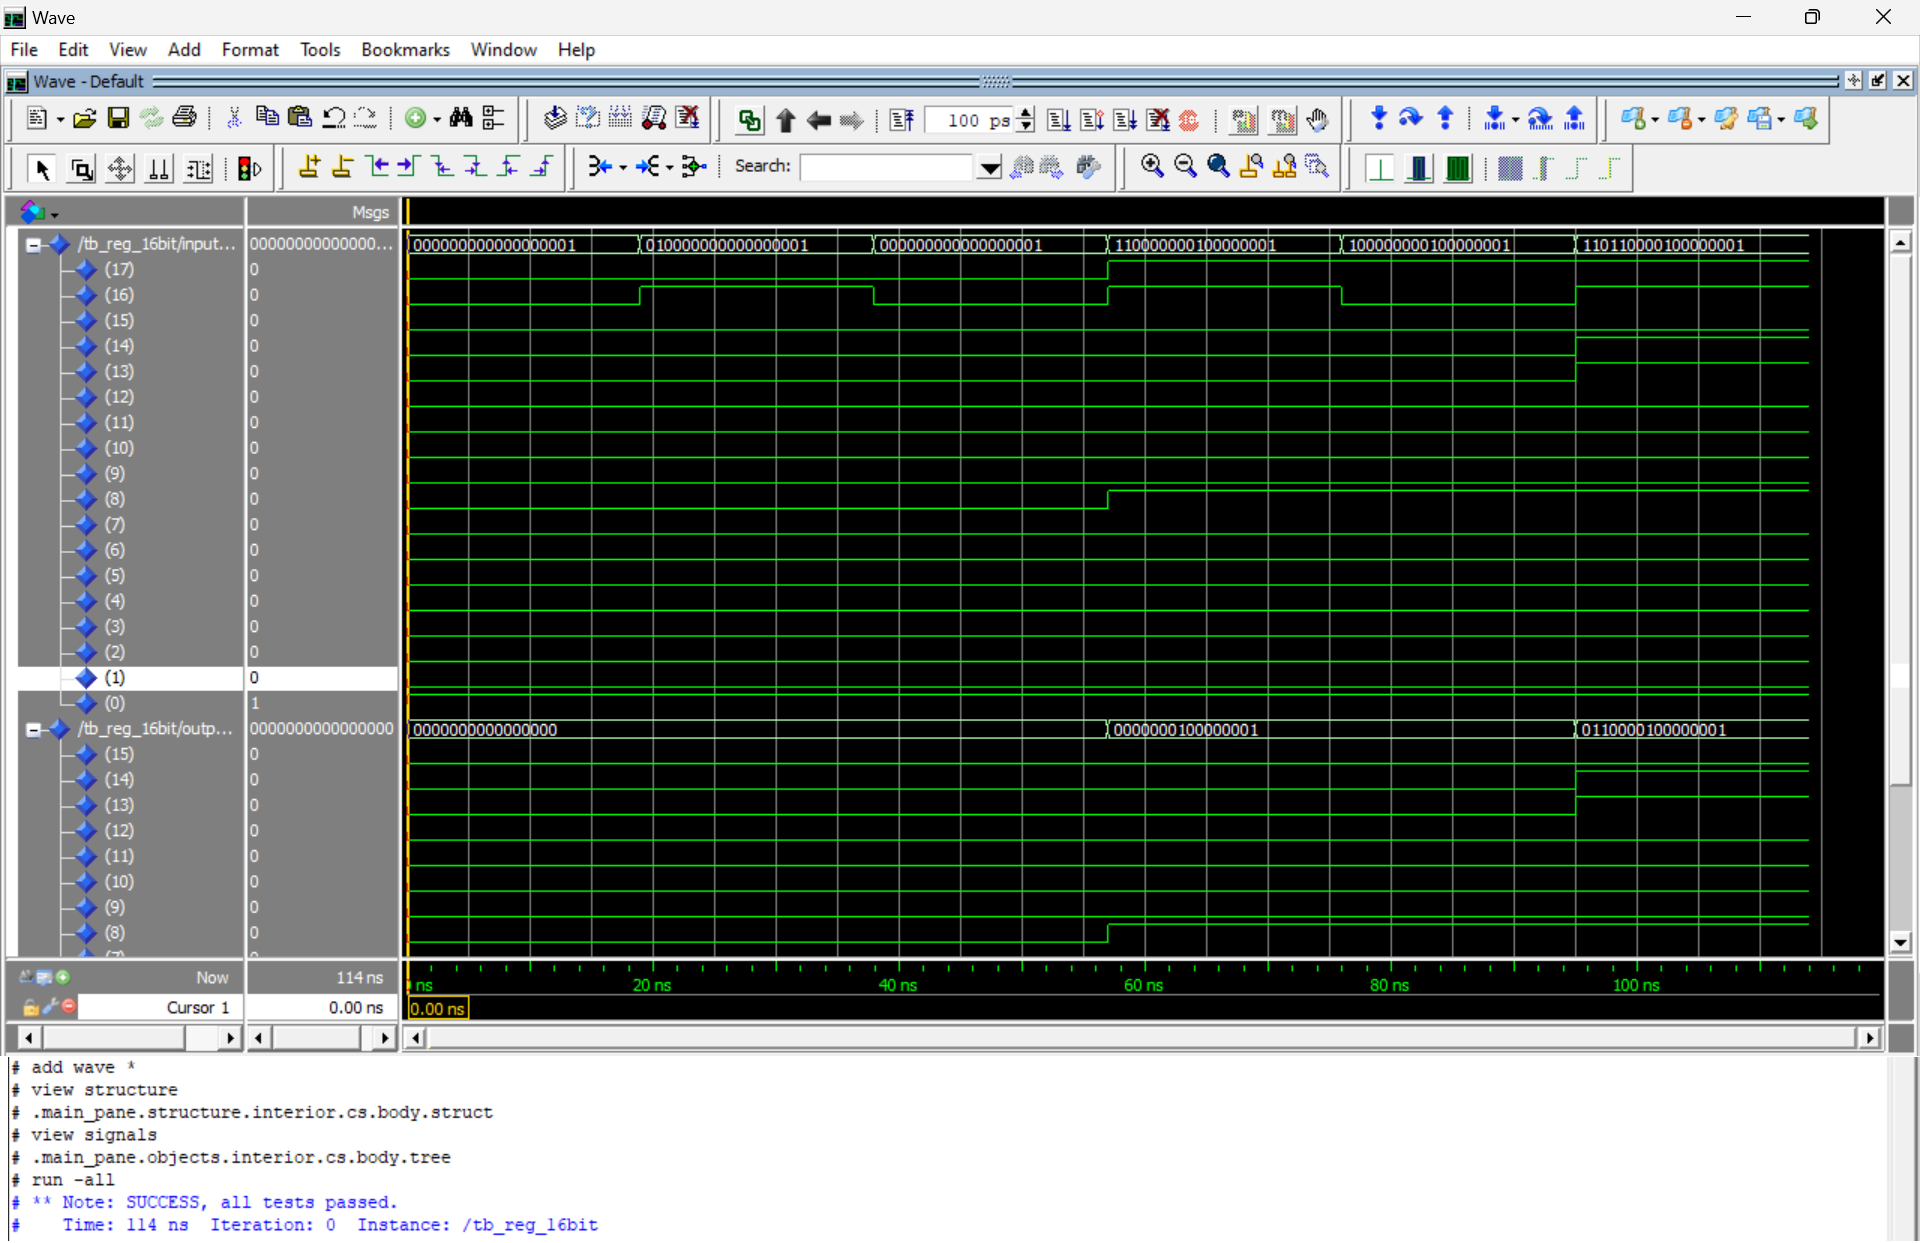
\includegraphics[width=\linewidth]{Images/sim_Reg_16BIT.png}
                \end{center}
                \caption{Simulation showing the perfect functioning of a 16-bit Register}
            \end{minipage}%
            }
    \end{figure}

    \begin{figure}
        \fbox{%
            \begin{minipage}{0.8\linewidth}
                \begin{center}
                    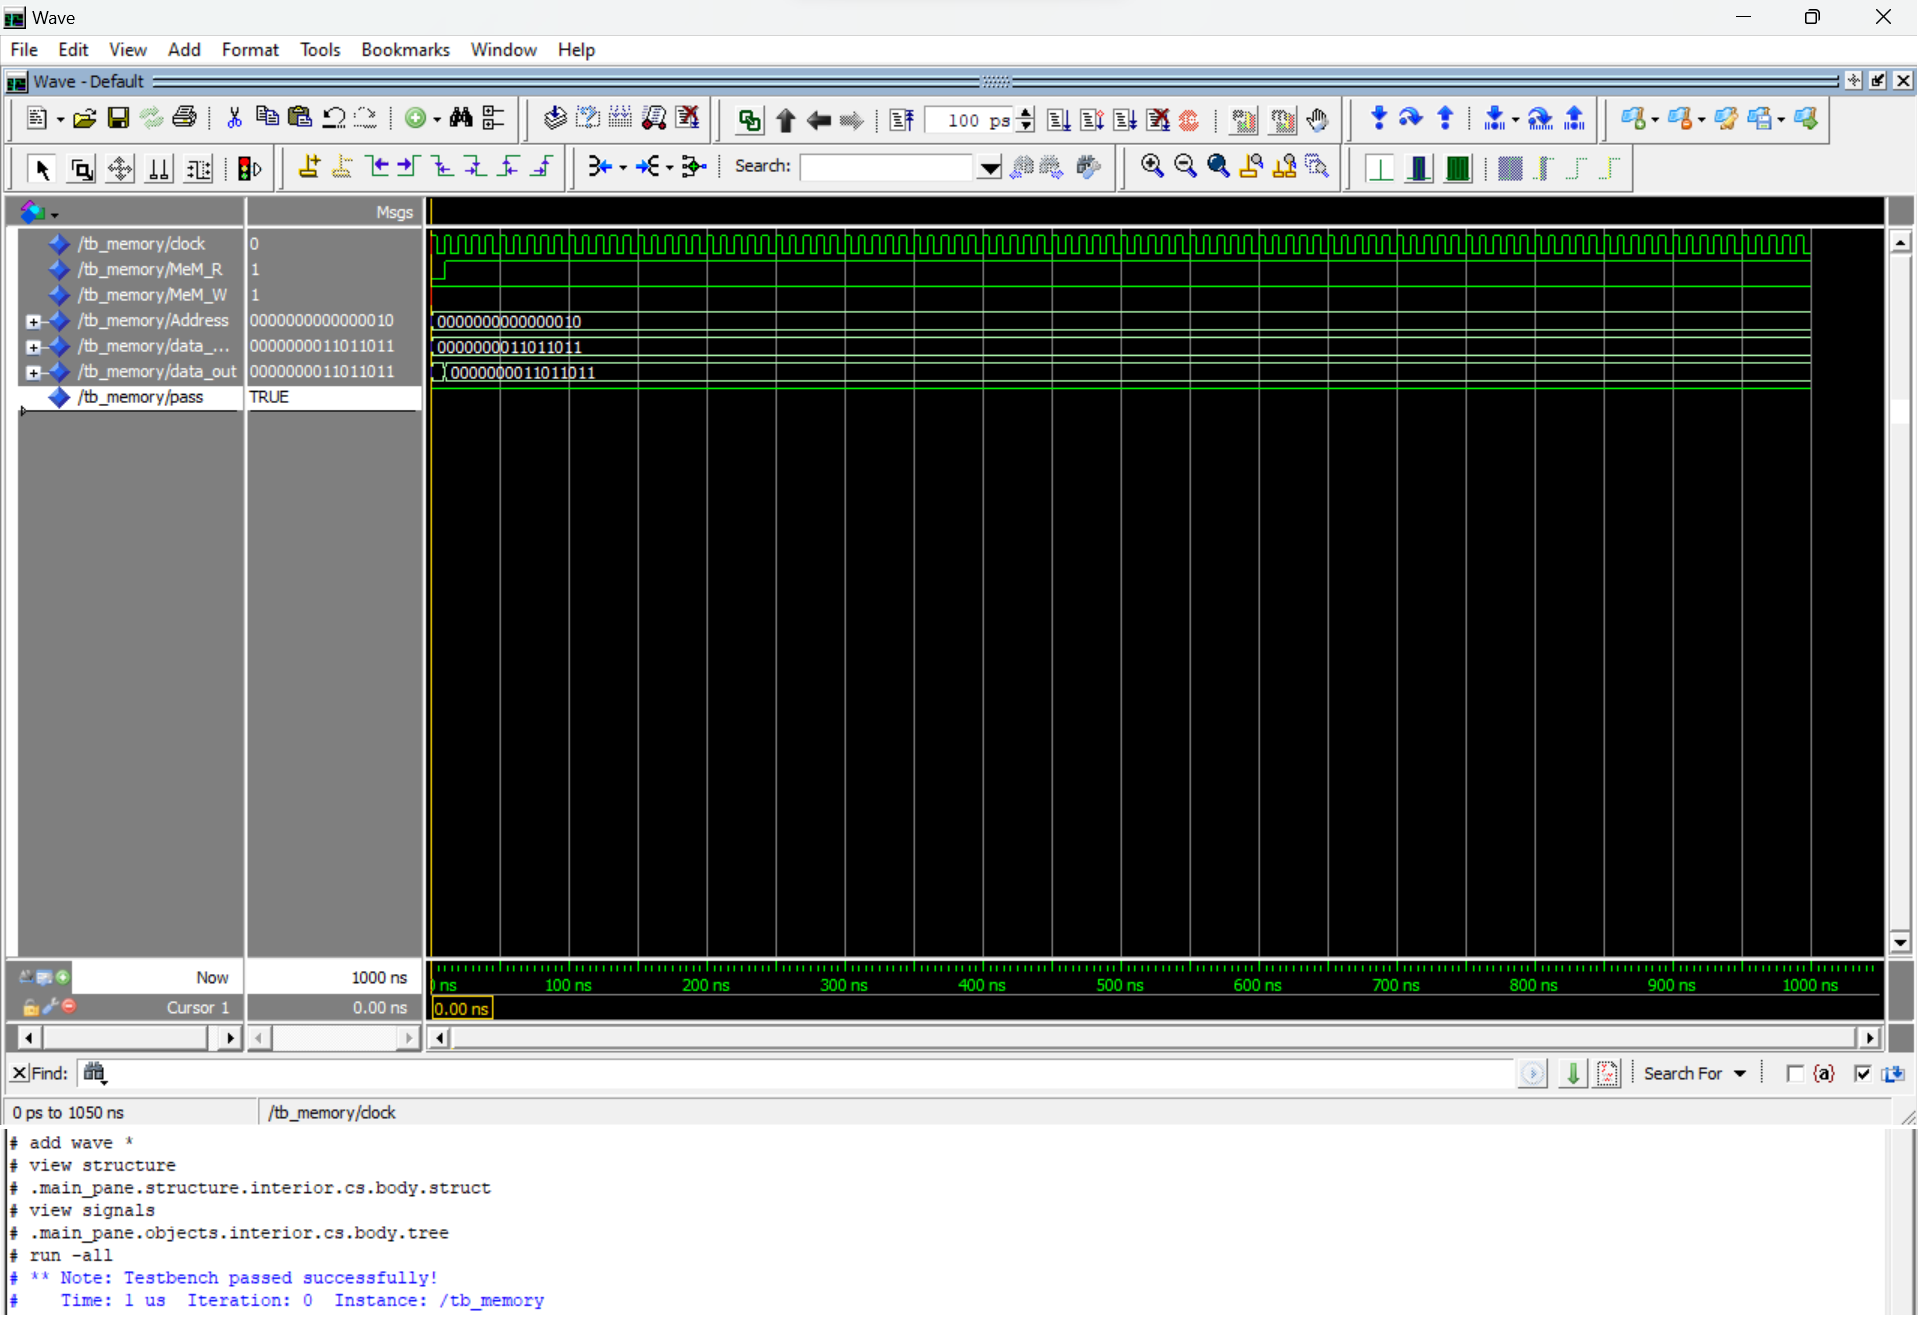
\includegraphics[width=\linewidth]{Images/Sim_Memory.png}
                \end{center}
                \caption{Simulation showing the perfect functioning of entity 'Memory'}
            \end{minipage}%
            }
    \end{figure}
\newpage
    \begin{figure}
        \fbox{%
            \begin{minipage}{0.9\linewidth}
                \begin{center}
                    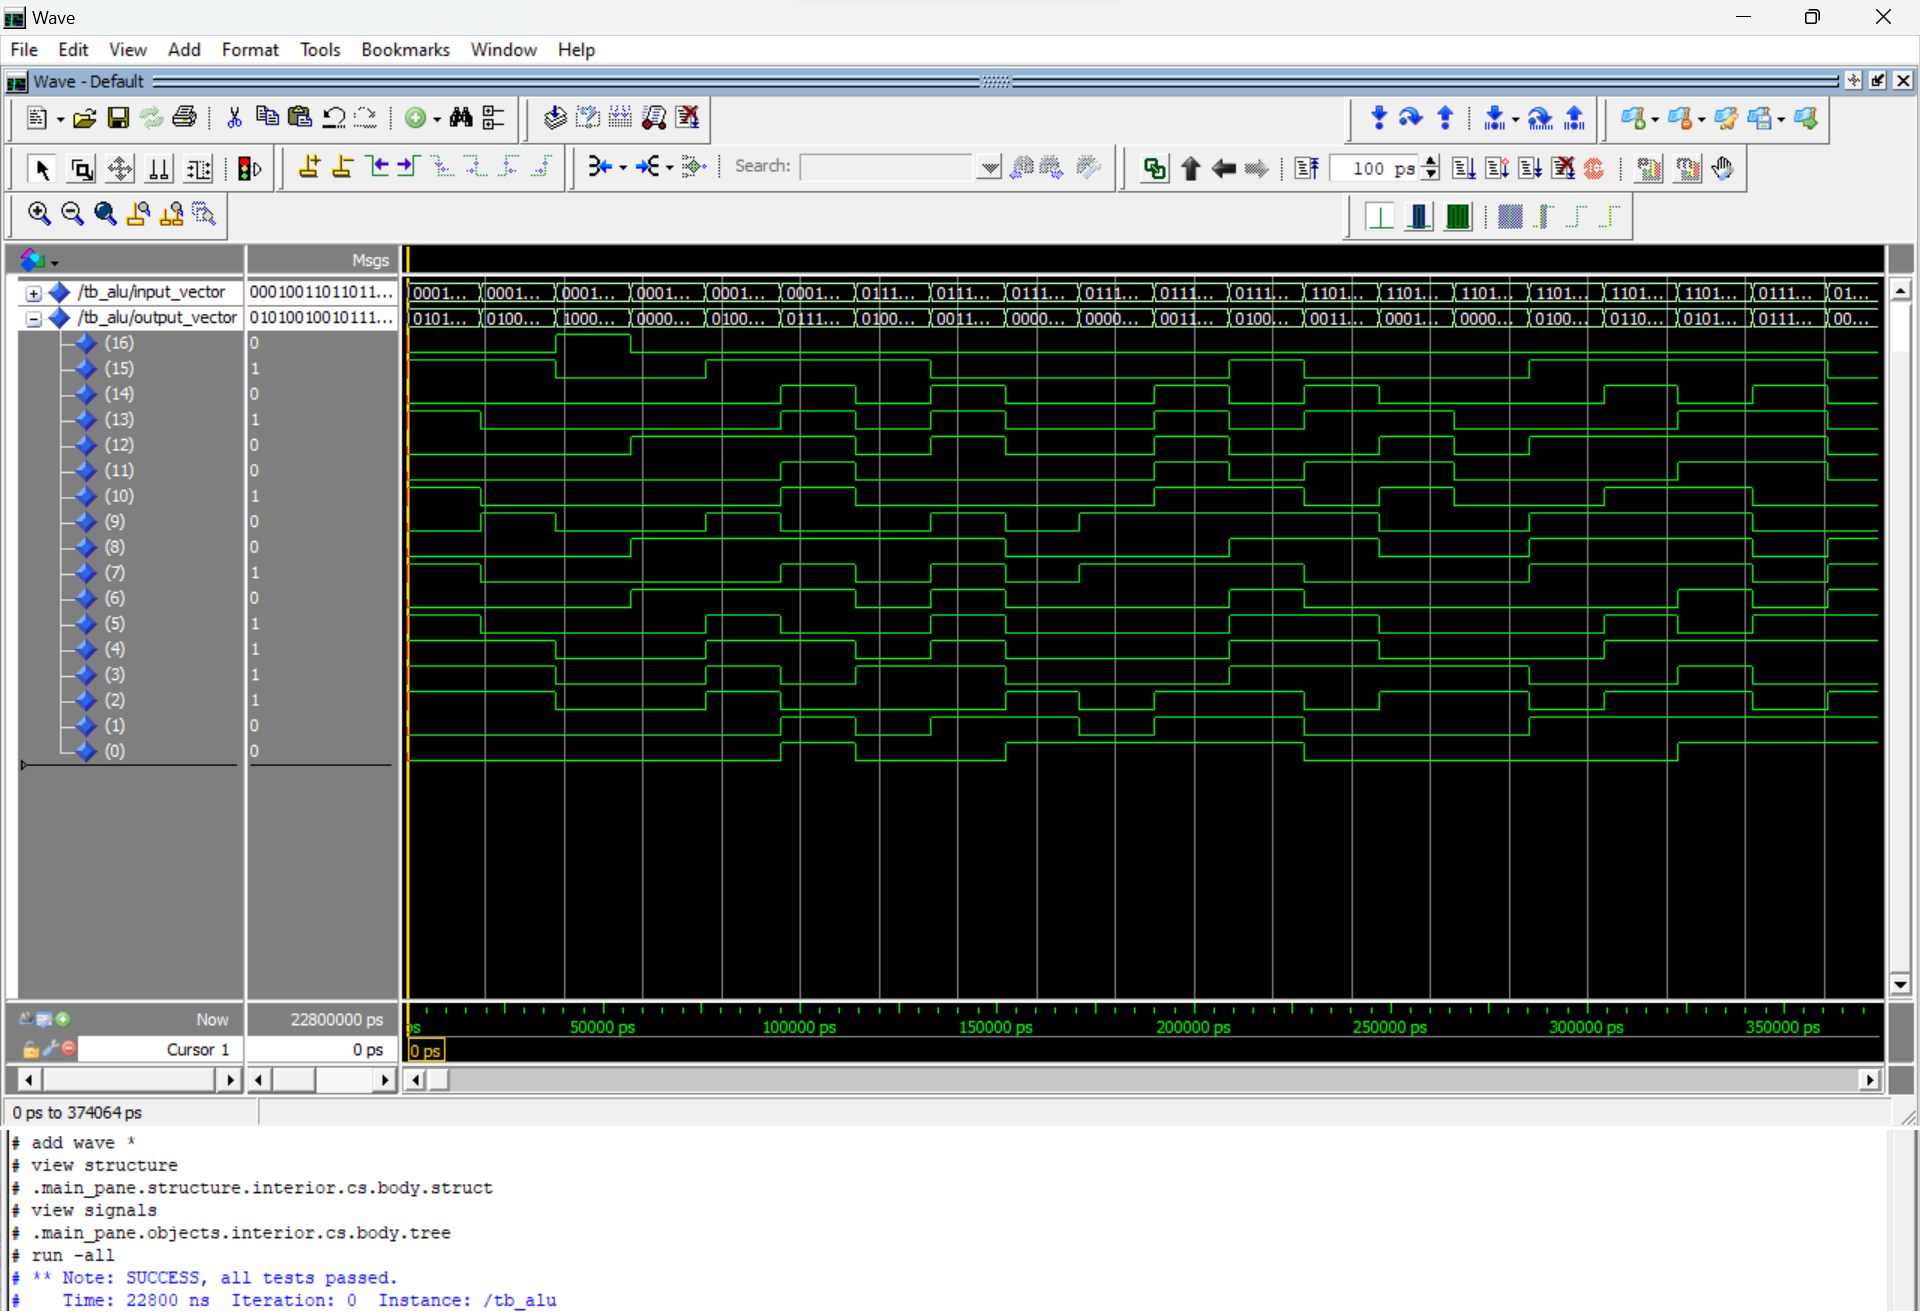
\includegraphics[width=\linewidth]{Images/Sim_ALU.png}
                \end{center}
                \caption{Simulation showing the perfect functioning of ALU that passed its generic Testbench}
            \end{minipage}%
            }
    \end{figure}

    \begin{figure}
        \fbox{%
            \begin{minipage}{1.01\linewidth}
                \begin{center}
                    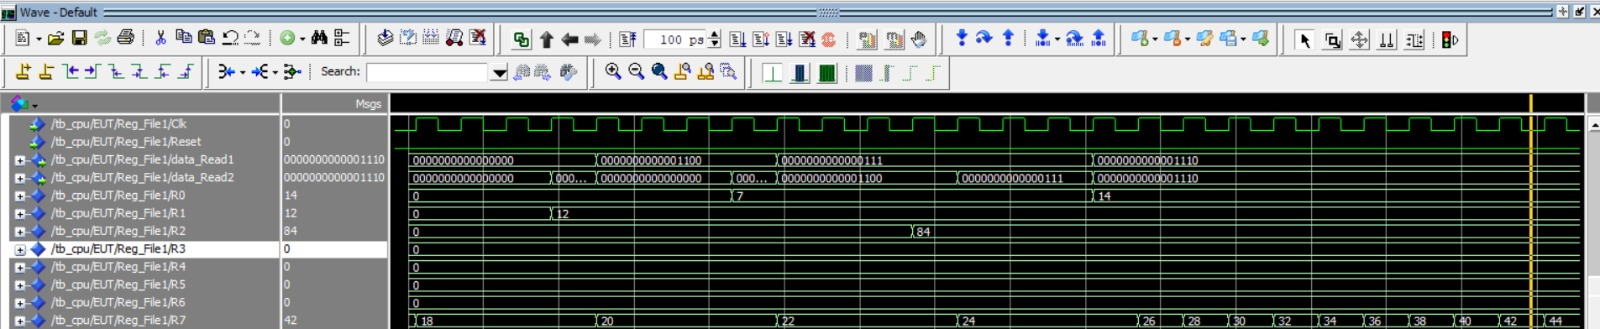
\includegraphics[width=\linewidth]{Images/Sim_ADI-ADI-MUL.png}
                \end{center}
                \caption{Test Case 1: \texttt{ADI-ADI-MUL}}
            \end{minipage}%
            }
    \end{figure} 

\clearpage
\newpage
\section{Datapath}
    \begin{raggedleft}
    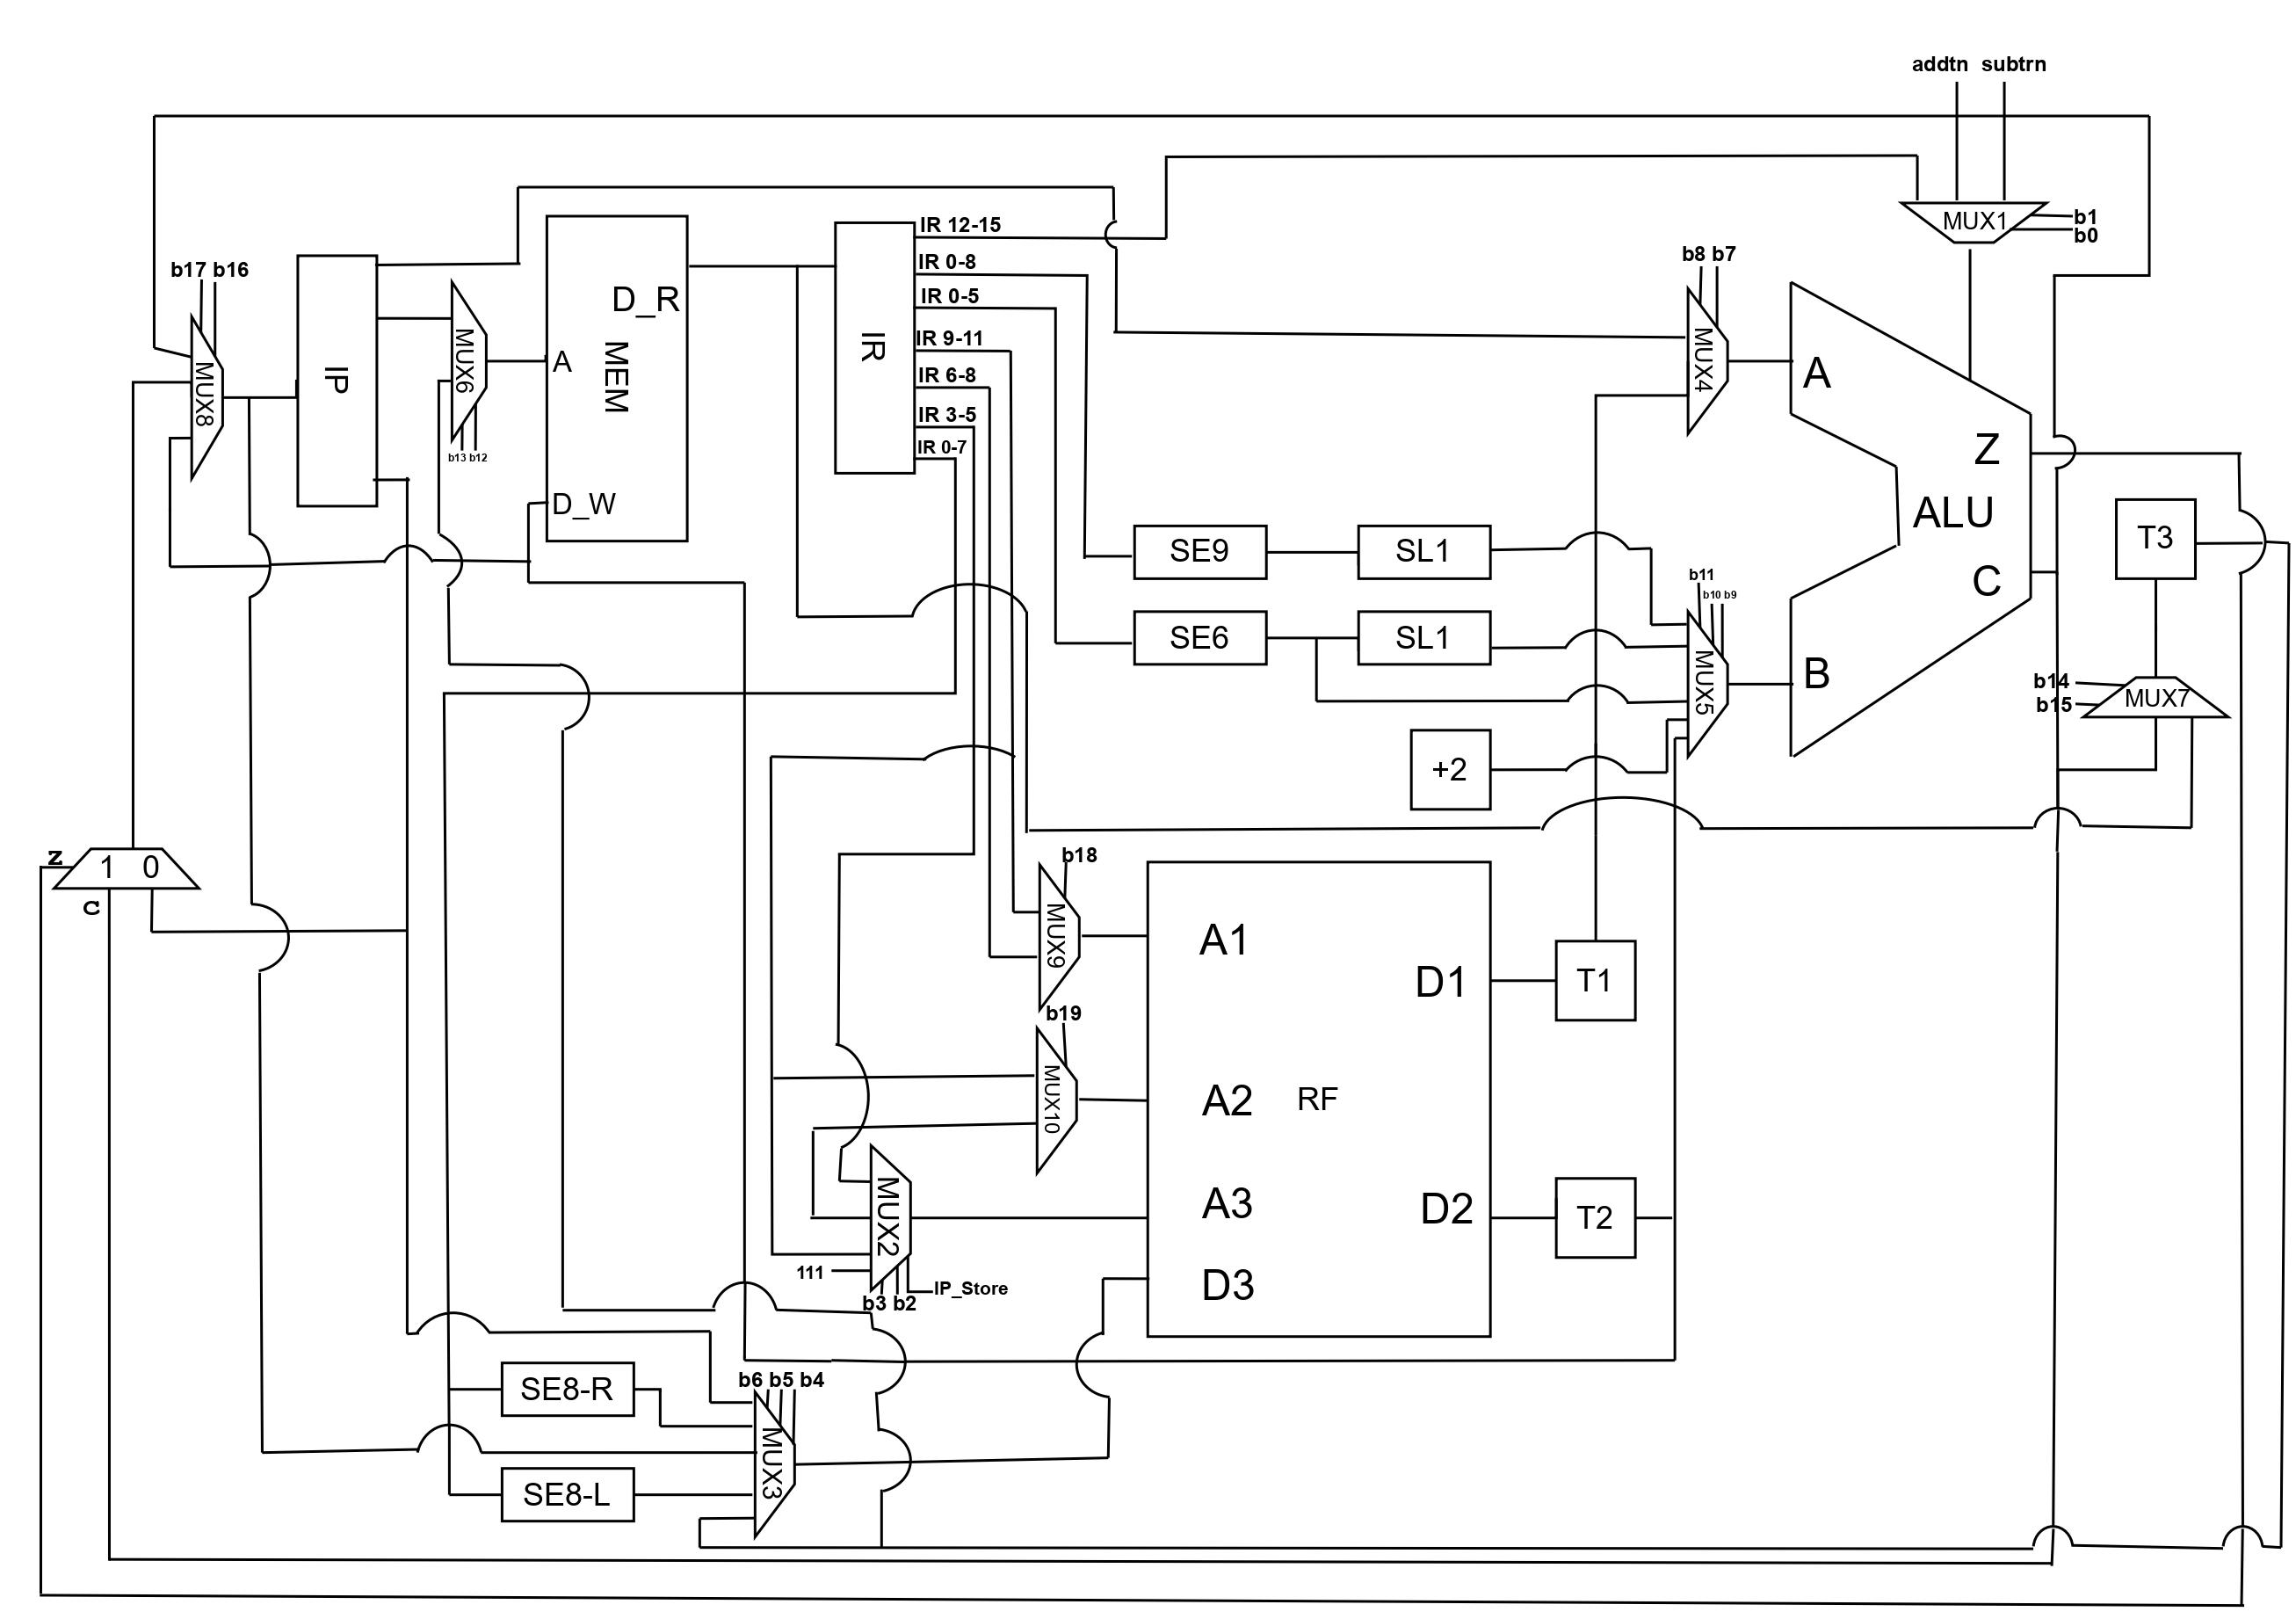
\includegraphics[width = 0.89\linewidth]
    {Images/iitb_cpu.jpg}
    \end{raggedleft}  
\section{Conclusion}
\begin{enumerate}
\item We have synthesized a General Fabric called CPU, which consists of a processing unit and a Memory. It has been created by orchestrating an Datapath which is controlled by a Controller. The Input to the CPU is a program and data (Depicted as a sequence of instructions hard coded into our memory).
\item The CPU in use interfaces with a randomly designated memory location, providing the flexibility to select any memory address for the input and output processes. This design allows for the writing of instructions and the observation of corresponding data outputs.
\item Our Datapath architecture consists of various components such as Registers, a Register File, Memory, Arithmetic Logic Unit (ALU) and Multiplexers. Our Control Logic maps out a Finite State Machine (FSM) which changes state every clock pulse based on the Instruction that has to be performed (Decoder Implementation). It is a \textbf{MULTI-CYCLE IMPLEMENTATION} to reduce the amount of hardware used.
\item Our Instruction Set Architecture (ISA) consists of a set of 14 instructions which the processor/computer architecture supports. This is a smaller set of simple instructions and hence is called \textbf{Reduced Instruction Set Computing (RISC)}.  The implementation of this ISA has been completely tested and verified via RTL simulations and signal analysis.
\item This Instruction set comprised of: \\
a) Arithmetic and Logical Instructions \texttt{(ADD,SUB,MUL,ADI,AND,ORA,IMP)}\\
b) Data Transfer Instructions \texttt{(LHI,LLI,LW,SW)}\\
c) Control Transfer Instructions \texttt{(BEQ,JAL,JLR)}
\item The specific details of the logic inside the processes (\texttt{state\_transition\_proc}, \texttt{output\_proc}, and multiplexer processes) determiness the exact behavior and functionality of the CPU.
\end{enumerate}

\end{document}
